
\chapter{Оптимизация расписания мультипроцессорного расписания и интервальная раскрашиваемость двудольных графов малого порядка}\label{AKM_ch1}



\section{Интервальная раскраска графов}\label{AKM_ch1_1}

%Исследования в области теории расписаний приводят к появлению новых методов и даже целых
%направлений в теории графов. Например, знаменитая проблема четырех красок возникла в связи с задачами теории расписаний
%и разбиений \cite[c. 101]{AKM_ch1_bib1}. В свою очередь, с проблемой четырех красок связана задача о правильной вершинной раскраске
%графа в три цвета, т.е. задача о существовании такого отображения множества вершин графа в множество цветов \{1, 2,
%3\}, что концевым вершинам каждого ребра сопоставляются разные цвета. Задача раскраски графа в три цвета
%$\mathit{NP}${}-полна \cite[c. 101]{AKM_ch1_bib1}, следовательно, не может быть разрешима за полиномиальное время, если верна знаменитая
%гипотеза <<$NP\neq P$>> (отметим недавнее сообщение Норберта Блюма о доказательстве данной гипотезы \cite{AKM_ch1_bib2} и
%работу \cite{AKM_ch1_bib3}).

Некоторые задачи теории расписаний представляется естественным формулировать в терминах \textit{реберной} раскраски.
Раскраску множества ребер  $E$  будем называть правильной реберной раскраской графа  $G=(V,E)$, если в каждой вершине
все \textit{представленные} \textit{в ней цвета} (цвета всех инцидентных ребер) различны. Следуя работе \cite{AKM_ch1_bib4},
\textit{интервальной t-раскраской} графа  $G=(V,E)$  будем называть правильную раскраску ребер  $G$  в цвета
$1,2,\dots ,t$, при которой в каждый цвет окрашено хотя бы одно ребро, а для каждой вершины  $v\in V$  ребра,
инцидентные  $v$, окрашены в  $d(v)$ \ последовательных цветов. Всюду в дальнейшем рассматриваются только реберные
раскраски. Если при каком-либо  $t$ \ граф имеет интервальную  $t${}-раскраску, будем говорить, что граф
\textit{интервально раскрашиваем}. В \cite{AKM_ch1_bib4} доказано, что задача об интервальной раскрашиваемости  $\mathit{NP}${}-полна.

Пусть планируется обработать множество заданий  $X=\{x_0,\dots ,x_{n-1}\}$  в системе специализированных процессоров
$Y=\{y_0,\dots ,y_{m-1}\}$; для каждого задания  $x_i$ \ определен набор процессоров, каждый из которых должен
выполнить одну операцию по обработке  $x_i$; длительность операции равна единице, запрещено одновременное участие
объекта (задания, процессора) в двух и более операциях, условия предшествования отсутствуют. Требуется выяснить,
существует ли расписание выполнения обработки без простоев объектов.

Рассмотрим двудольный граф  $G=\left(X,Y,E\right)$, где  $\left(x_i,y_j\right)\in E$, если и только если процессору
$y_j$ \ предписано выполнить операцию над заданием  $x_i$. Под расписанием длины  $t$ \ будем понимать отображение
множества ребер  $E$ \ в множество  $\{1,2,\dots ,t\}$, где каждому ребру  $\left(x_i,y_j\right)\in E$
\ сопоставляется  $c\left(x_i,y_j\right)$\ - номер дискретного момента времени, в течение которого  $y_j$ \ выполняет
операцию над  $x_i$. Если рассматривать  $c(x_i,y_j)$ \ в качестве цвета ребра $(x_i,y_j)$, получим эквивалентную
задачу интервальной реберной раскраски двудольного графа. Запрет на одновременное участие объекта в двух и более
операциях в терминологии теории графов означает, что раскраска должна быть \textit{правильной}, а отсутствие простоев ---
что раскраска должна быть и \textit{интервальной}, т.е. в каждой вершине графа все представленные в ней цвета должны
образовать целочисленный интервал (всюду в дальнейшем под интервалом будем понимать целочисленный интервал, интервал
$\{a,a+1,\dots ,b\}$ будем обозначать $[a..b]$). В \cite{AKM_ch1_bib5} показано, что задача об интервальной раскрашиваемости
заданного двудольного графа  $\mathit{NP}${}-полна.

\section{Свойства интервальной раскраски}\label{AKM_ch1_2}

\ Естественно ожидать, что двудольные графы с малым порядком интервально раскрашиваемы. Возникает вопрос: <<Каково самое
сильное ограничение на количество вершин, при котором задача все еще остается NP-полной?>> С применением компьютерных
ресурсов в \cite{AKM_ch1_bib6} доказано следующее утверждение.

\begin{statement}\label{AKM_ch1_s1}
	Все двудольные графы с числом вершин не более 14 интервально раскрашиваемы.
\end{statement}

В ряде статей (например, в \cite{AKM_ch1_bib7}) указывается, что вопрос интервальной раскрашиваемости двудольных графов порядка 15, 16,
17 и 18 остается открытым.

\begin{corollary}
	Если двудольный граф  $G=(X,Y,E)$ \ с числом вершин 15 несвязен или обладает висячим ребром, то граф  $G$
	\ интервально раскрашиваем.
\end{corollary}

Интересно, что и малая мощность только одной доли способна обеспечить двудольному графу  $G=(X,Y,E)$ \ интервальную
раскрашиваемость.


\begin{statement}[\cite{AKM_ch1_bib8}]\label{AKM_ch1_s2}
	Если для двудольного графа  $G=(X,Y,E$) выполнены неравенства  $\left|X\right|\leq 3$ или
	$\left|Y\right|\leq 3$, то граф  $G$ \ интервально раскрашиваем.
\end{statement}
%Утверждение 2 [8].

\begin{statement}\label{AKM_ch1_s3}
	Пусть задана интервальная раскраска связного графа и
	
	\begin{equation*}
	P=(a_0,b_0,a_1,b_1,\dots ,b_{n-1},a_n)
	\end{equation*}
	- цепь, соединяющая два ребра:  $b_0=(a_0,a_1)$ \ и  $b_{n-1}=(a_{n-1}$,  $a_n$) с цветами  $t_0$ \ и  $t_{n-1}$
	\ соответственно,  $t_0<t_{n-1}$. Тогда для любого  $\tau $,  $t_0<\tau <t_{n-1}$, найдется ребро цвета  $\tau $,
	инцидентное некоторой вершине из  $P$.
\end{statement}

%\begin{proof}
%	Обозначим интервал цветов, представленных в вершине  $a_i$, через  $[m_i..M_i]$;  $m'=\underset
%	i{\mathit{min}}m_i,M'=\underset i{\mathit{max}}M_i$. Т.к. каждые два соседних интервала последовательности
%	
%	\begin{equation*}
%	\left[m_0..M_0\right],\left[m_1..M_1\right],\dots ,[m_{n-1}..M_{n-1}]
%	\end{equation*}
%	имеют непустое пересечение, то каждый цвет из интервала $[m'..M']$ представлен в некоторой вершине цепи  $P.$
%	\ Поскольку  $t_0\in \left[m_0..M_0\right],t_{n-1}\in \left[m_{n-1}..M_{n-1}\right],$ \ то
%	$t_0,t_{n-1}\in \left[m'..M'\right];$ \ следовательно, и  $\tau \in \left[m'..M'\right],$ \ поэтому цвет  $\tau $
%	\ представлен в некоторой вершине цепи  $P.$\ ${\blacksquare}$
%\end{proof}

Из Утверждения \ref{AKM_ch1_s3} немедленно вытекает следующее утверждение.

\begin{statement}\label{AKM_ch1_s4}
	Приведенное выше определение интервальной  $t${}-раскраски из работы [?] равносильно следующему:
	<<Интервальной  $t${}-раскраской связного графа  $G$  называется раскраска ребер  $G$  в цвета  $1,2,\dots ,t$, при
	которой найдутся ребра, окрашенные в цвета  $1$  и  $t$, и для каждой вершины  $v$  цвета, представленные в  $v$,
	образуют множество последовательных чисел>>.
\end{statement}

\begin{statement}[\cite{AKM_ch1_bib4}]\label{AKM_ch1_s5}
	Если двудольный граф на  $k$  вершинах обладает интервальной  $t${}-раскраской, то  $t \leq k-1$.
\end{statement}
%Утверждение 5. [4]

Двудольный граф  $G=(X,Y,E)$, где  $\left|X\right|=n$, $\left|Y\right|=m,$ \ будем называть  $(n,m)${}-\textit{графом}.
Подход, предложенный в следующих разделах, в частности, позволил доказать, что все  $(n,m)$-\linebreak графы порядка 15
интервально раскрашиваемы.

\section{Перечисление нормализованных $(n,m)$-графов}\label{AKM_ch1_3}
\hypertarget{Toc503377124}{}\textbf{Нормализованное представление двудольного графа}. Рассмотрим двудольный граф \linebreak
$G=(X,Y,E)$, где  $X=\{x_0,\dots,x_{n-1}\}$,  $Y=\{y_0,\dots,y_{m-1}\}$.

Подмножество вершин  $Y$, смежных (не смежных) вершине  $x_i\in X$, обозначим через  $Y_i(\bar{Y}_i)$;
$i=0,\dots ,n-1$.  Множество индексов вершин подмножества  $Z \subset Y$, образованного последовательными вершинами
из множества  $Y$, будем называть \textit{индексным интервалом} множества  $Z$. Введем понятие \textit{нормализованного
	представления} графа  $G=(X,Y,E)$.

\noindent\textbf{1.} Автоморфизмом множества  $Y$  разместим вершины множества  $Y_0$  в начальных позициях множества  $Y$. Тем
самым интервал [$0..n-1$] разбивается на индексные интервалы множеств  $Y_0$ \ и  $\bar{Y}_0$.

\noindent\textbf{2.} Пусть  $0<i<n-1$  и в результате некоторого автоморфизма  $\alpha $  интервал [$0 .. n-1$] разбит на  $2^i$
\ последовательных интервалов --- индексных интервалов некоторых множеств  $Z_0,\dots ,Z_{2^i-1}$, некоторые из которых
могут быть пустыми. Выполним для каждого  $Z_j$  автоморфизм  $\beta _j$, размещающий все вершины множества  $Z_jY_i$
\ в начальных позициях множества  $Z_j$, а вершины множества  $Z_j\bar{Y}_i$ --- соответственно в последних позициях
множества  $Z_j$. Суперпозицию  $\alpha {\cdot}\beta _0{\cdot}\dots {\cdot}\beta _{2^i-1}$  снова обозначим через
$\alpha $. Автоморфизм  $\alpha $  индуцирует разбиение интервала [$0..n-1$] на  $2^{i+1}$  последовательных
интервалов --- индексных интервалов множеств

\begin{equation}\label{AKM_ch1_e1}
Z_0\bigcap Y_i, Z_0\bigcap \bar{Y}_i,\dots , Z_{2^i-1}\bigcap Y_i, Z_{2^i-1}\bigcap \bar{Y}_i.
\end{equation}

Увеличим  $i$ \ на единицу и переобозначим множества \eqref{AKM_ch1_e1} через  $Z_0,\dots ,Z_{2^i-1}$ \ последовательно слева-направо.

Пока  $i<n-1$, повторим выполнение пункта \textbf{2}, по достижении равенства  $i=n-1$ \ перенумеруем вершины множества
$X$ \ по невозрастанию их степеней:

\begin{equation}\label{AKM_ch1_e2}
d\left(x_0\right)\geq d\left(x_1\right)\geq \dots d(x_{n-1})
\end{equation}

и полученный граф назовем \textit{нормализованным графом }или --- если необходимо подчеркнуть связь с графом
$G=(X,Y,E)$\ --- \textit{нормализованным представлением графа}  $G=(X,Y,E)$.

\section{Схема перечисления нормализованных ($n,m$)-графов}\label{AKM_ch1_4}
\hypertarget{Toc503377125}{}В данном разделе приведено развернутое изложение идеи работы [9]. Значение
\foreignlanguage{english}{\textit{p}} всюду в дальнейшем выбирается равным 15 или 16. Очевидно, граф  $G=(X,Y,E)$
\ изоморфен своему нормализованному представлению. Поэтому достаточно проверить интервальную раскрашиваемость всех
нормализованных ($n,m$)-графов. Несмотря на то, что среди них могут встретиться изоморфные графы, компьютерный перебор
всех нормализованных ($n,m$)-графов потребует при  $n+\text{~}m=p$\ <<значительно меньше>> времени, нежели перебор всех
($n,m$)-графов. Существенному сокращению времени перебора призвано способствовать и то обстоятельство, что мы
ограничимся связными графами без висячих вершин (см. следствие Утверждения \ref{AKM_ch1_s1}) и случаем  $3<\text{~}n$\ (см.
Утверждение \ref{AKM_ch1_s2}).

\begin{remark}\label{AKM_ch1_r1}
	Задача об изоморфизме графов является <<открытой>> задачей, относительно которой неизвестно, является ли она
	$\mathit{NP}${}-полной.
\end{remark}

При реализации алгоритма в многократных внутренних итерациях очередного вложенного цикла по  $i=0,\dots ,n-1$
\ используются целочисленные переменные  $a_{\mathit{ij}}$, которые пробегают значения из соответствующих индексных
интервалов (на рис.~1.1 - наименьшие по длине интервалы, охватывающие  $a_{\mathit{ij}}$), формируются суммы

\begin{equation*}
d(x_i)=a_{i0}+a_{i1}+\dots +a_{i,2^i-1}
\end{equation*}
и, если неравенство \eqref{AKM_ch1_e2} выполнено, то  $d(x_i)$ \ вершин множества  $Y$ \ с соответствующими индексными интервалами
длины  $a_{\mathit{ij}}$ \ выбираются в качестве вершин, смежных вершине  $x_i$ $(i=0,\dots ,n-1)$.

Схема перечисления всех нормализованных ($n,m$)-графов представлена на рис.\ref{AKM_ch1_img1} (ввиду очевидной проблемы отображения
деталей рисунок приведен для случая \foreignlanguage{english}{\textit{p}}\textit{=15}, распространение на случай
\foreignlanguage{english}{\textit{p}}\textit{=16} тривиально). Продемонстрируем на примерах использование этой схемы.

\begin{example}\label{AKM_ch1_ex1}
	Генерация списков смежности для вершины  $x_3$.
\end{example}

\  $d(x_3)=a_{30}+a_{31}+a_{32}+a_{33}$+ $a_{34}+a_{35}+a_{36}+a_{37}$. В список вершин, смежных  $x_3$, выбираются по
$a_{3j}$ \ вершин множества  $Y$, индексы которых - суть  $a_{3j}$ значений из начала интервала  $Z_{3j}$,
$j=0,\dots ,7$, где:

$Z_{30}=$[ $0..a_{20}-1$],  $Z_{31}=$[ $a_{20}..a_{10}-1$],  $Z_{32}=$[ $a_{10}..a_{10}+a_{21}-1$],  $Z_{33}=$[
$a_{10}+a_{21}..a_0-1$],  $Z_{34}=$[ $a_0..a_0+a_{22}-1$],

$Z_{35}=$[ $a_0+a_{22}..a_0+a_{11}-1$],  $Z_{36}=$[ $a_0+a_{11}..a_0+a_{11}+a_{23}-1$],  $Z_{37}=$[
$a_0+a_{11}+a_{23},\dots ,m-1$].

\begin{figure}[H]\label{AKM_ch1_img1}
	\centering
	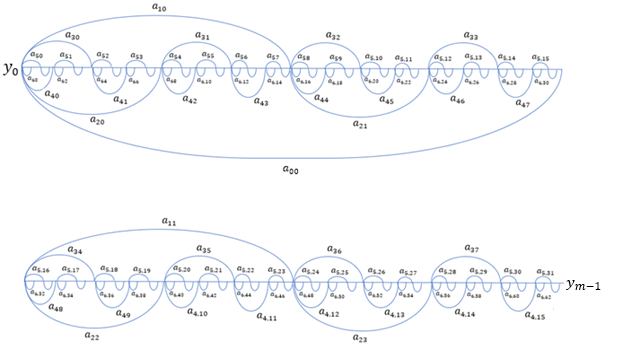
\includegraphics[width=1\textwidth]{AM/1}
	\caption{Схема генерации всех нормализованных $(n,m)$-графов, $n \leq 7$; нижняя часть рисунка является непосредственным продолжением верхней части. При $n<7$ рисунок корректируется путем удаления всех интервалов, обозначенных $a_{ij},i>n-1$}
\end{figure}

\begin{example}\label{AKM_ch1_ex2}
	Генерация списков смежности для вершины  $x_4$.
\end{example}

$d(x_4)=a_{40}+a_{41}+a_{42}+a_{43}$+ $a_{44}+a_{45}+a_{46}+a_{47}$+ $a_{48}+a_{49}+a_{4,10}+a_{4,11}$+
$a_{4,12}+a_{4,13}+a_{4,14}+a_{4,5}$. В список смежных  $x_4$ \ вершин будем выбирать по  $a_{4j}$ \ вершин множества
$Y$ \ с индексами из начала интервала  $Z_{4j}$,  $j=0,\dots ,15$, где:

$Z_{40}=$[ $0..a_{30}-1$],  $Z_{41}=$[ $a_{30}..a_{20}-1$],  $Z_{42}=$[ $a_{20}..a_{20}+a_{31}-1$],  $Z_{43}=$[
$a_{20}+a_{31}..a_{10}-1$],  $Z_{44}=$[ $a_{10}..a_{10}+a_{32}-1$],

$Z_{45}=$[ $a_{10}+a_{32}..a_{10}+a_{21}-1$],  $Z_{46}=$[ $a_{10}+a_{21}..a_{10}+a_{21}+a_{33}-1$],

$Z_{47}=$[ $a_{10}+a_{21}+a_{33}..a_0-1$],  $Z_{48}=$[ $a_0..a_0+a_{34}-1$],

$Z_{49}=$[ $a_0+a_{34}..a_0+a_{22}-1$],  $Z_{10}=$[ $a_0+a_{22}..a_0+a_{22}+a_{35}-1$],  $Z_{4,11}=$[
$a_0+a_{22}+a_{35}..a_0+a_{11}-1$],  $Z_{4,12}=$[  $a_0+a_{11}..a_0+a_{11}+a_{36}-1$],

$Z_{4,13}=$[ $a_0+a_{11}+a_{36}..a_0+a_{11}+a_{23}-1$],

$Z_{4,14}=$[ $a_0+a_{11}+a_{23}..a_0+a_{11}+a_{23}+a_{37}-1$],

$Z_{4,15}=$[ $a_0+a_{11}+a_{23}+a_{37}..m-1$].

Справедливость следующего утверждения очевидна.

\begin{statement}\label{AKM_ch1_s6}
	Пусть  $S$\ - множество всех связных $(n,m)$-графов без висячих вершин,  $S_0$\ - множество всех
	нормализованных $(n,m)$-графов. Для каждого графа  $G$ \ из  $S$ \ в множестве  $S_0$ \ найдется граф, изоморфный
	графу  $G$.
\end{statement}

\section{Жадный алгоритм интервальной раскраски}\label{AKM_ch1_5}
\hypertarget{Toc503377126}{}\textbf{Кусочно-непрерывный путь в связном графе}. В разделе \ref{AKM_ch3_2} изложена модификация
жадного алгоритма проверки интервальной раскрашиваемости, приведенного в \cite{AKM_ch1_bib10}. В формулировке алгоритма используется
понятие \textit{кусочно-непрерывного пути} в графе  $G$. Приведем логическую (с результатом
\foreignlanguage{english}{\textit{True}} или \foreignlanguage{english}{\textit{False}}) процедуру генерации
кусочно-непрерывного пути.

Пусть в графе  $G$ \ выбрана произвольная непродолжимая цепь  $P$ \ и логической переменной
\foreignlanguage{english}{\textit{Result}} присвоено значение \foreignlanguage{english}{\textit{True}}.

\textbf{Пока} не все ребра графа  $G$ \ включены в  $P,$ \ выполним следующие три действия:
\begin{enumerate}[1)]
  \item
если среди вершин цепи
$P$ \ найдется вершина с инцидентным ребром, не включенным в  $P$, то последнюю из таких вершин обозначим  $a_k$ \ и
перейдем к второму действию, в противном случае присвоим переменной \foreignlanguage{english}{\textit{Result}} значение
\foreignlanguage{english}{\textit{False}} и <<досрочно>> завершим цикл;
  \item
  построим непродолжимую цепь  $P_1$,
начинающуюся с вершины  $a_k$ \ и содержащую лишь ребра, не включенные в  $P$;
  \item
результат конкатенации  $P$ \ и $P_1$ \ обозначим снова через  $P$.
\end{enumerate}


Если по завершении цикла значение переменной \foreignlanguage{english}{\textit{Result}} равно
\foreignlanguage{english}{\textit{True}}, то последовательность ребер графа  $G$, перечисленных в том порядке, в каком
они следуют в итоговом  $P$, будем называть кусочно-непрерывным путем в графе  $G$, в противном случае заключаем, что
граф  $G$ \ не является связным и кусочно-непрерывный путь не существует.

\textbf{Жадный алгоритм }\textbf{интервальной раскраски. }Напомним, что требуется проверить, существует ли интервальная
раскраска заданного связного ($n,m$)-графа  $G=(X,Y,E)$ \ не более чем  $t$ \ цветами (и выполнить раскраску в случае
существования).

Количество вершин и ребер графа  $G$ обозначим через  $H$ и $h$ соответственно $(H=n+m)$. В соответствии с
Утверждением \ref{AKM_ch1_s5}, положим  $t$ \ равным  $H-1$\ (это единственный пункт алгоритма, учитывающий двудольную природу графа
$G$). Использованные далее обозначения, присущие языкам программирования, понятны без дополнительных объяснений.
Например,  $i$++ ($i${}-{}-) означает увеличение (уменьшение) значения переменной  $i$ на единицу, скобки  $\{\}$
\ используются для обозначения блока (группового оператора).

Построим кусочно-непрерывный путь  $P=\{e_0,\dots ,e_{h-1}\}$ \ и будем последовательно окрашивать ориентированные
ребра  $e_i=(v_i,w_i)$ цветами из целочисленного интервала  $[1..t]$ \ так, что в любой момент времени в каждой
вершине  $v$ \ представленные в  $v$ \ цвета образуют некоторый список  $L_v$, составленный из последовательных целых
чисел. Алгоритм раскраски, обладающий таким свойством, будем называть \textit{жадным алгоритмом}. Массив текущих
списков цветов, представленных в вершинах множества  $V$, будем обозначать через  $L$,
$L=\{L_{v_0},\dots ,L_{v_{H-1}}\}$. \textit{Приграничным цветом} для пустого интервала назовем любой цвет из интервала
$[1..t]$, для непустого интервала  $[a..b]$ \textit{\ нижним приграничным цветом} назовем цвет  $a-1$, если
$1\leq a-1\leq t$, \textit{верхним приграничным цветом} --- цвет  $b+1$, если  $1\leq b+1\leq t;$ \ в случае
существования, нижний и верхний приграничные цвета для списка  $L_{v_i}$  будем обозначать через
$\mathit{low}\left(v_i\right)$  и  $\mathit{high}(v_i)$ соответственно.

Рассмотрим ситуацию, когда ребра  $e_0, \dots ,e_{i-1}$ уже окрашены и требуется окрасить ребро  $e_i$,  $i>0$. Список
цветов в начальной вершине  $v_i$ ориентированного ребра  $e_i=(v_i,w_i)$ не пуст, так как содержит цвет ребра
$e_{i-1}$. Очевидно, что окраска ребра  $e_i$ \ без изменений цветов ранее окрашенных  $i$ \ ребер возможна только в
следующих двух случаях:
\begin{enumerate}[1)]
  \item
  $\mathit{low}(v_i)$ \ существует и является приграничным цветом для  $w_i$;
  \item
  $\mathit{high}(v_i)$ существует и является приграничным цветом для  $w_i$.
\end{enumerate}
Соответственно допустимы две попытки
окрасить ребро  $e_i$ без изменений цветов ранее окрашенных ребер; номера 1 или 2 предпринятых попыток будем
сохранять в ячейке  $q_i$ (удобно использовать и третье значение  $q_i=0$ в качестве признака, что ни одна из двух
попыток пока не предпринята).
 Заметим, что элементы массива  $q$  индексируются, начиная с единицы, в отличие от всех
других массивов, используемых в нашем алгоритме.

Для записи и хранения цвета ребра  $e_i$  будем использовать ячейку  $C_i$. В качестве признака успешного (с
построением интервальной раскраски) или неудачного (без построения интервальной раскраски) завершения жадного алгоритма
используется логическая переменная  $\mathit{Success}$.

Перейдем к изложению жадного алгоритма, который осуществляет перебор с возвратами и, кроме стадии инициализации,
включает итерации с двумя пунктами: <<Прямой шаг>> и <<Возвратный шаг>>.

1. Инициализация

$\mathit{Success}:=\mathit{false}$; всем  $v_i$\ (соответственно  $w_i$) присвоить номера начальных (конечных) вершин
ориентированных ребер  $e_i$ \ из кусочно-непрерывного пути  $P,i=\text{~}0,\dots ,h-\text{~}1;$ \ для всех вершин
выбрать пустые списки цветов:  $L_{v_0}:=\text{~}{\emptyset};$\  $\dots ;L_{v_{H-1}}:$= ${\emptyset};$ всем элементам
массивов  $q$ \ и  $C$ \ присвоить нулевые значения:  $q_1:=0;$\  $\dots ;q_{h-1}:=0;C_0:=0;\dots ;C_{h-1}:=0$;
начальное ребро  $e_0$ \ окрасить в цвет 1:  $C_0:=1$;  $L_{v_0}:=\left\{1\right\};L_{w_0}$ \  $=\left\{1\right\};$
номер очередного окрашиваемого ребра выбрать равным единице:  $i:=1$.

2. Прямой шаг

\foreignlanguage{english}{\textbf{FWRD}}: данный пункт выполняется сразу после инициализации или же после возвратного
шага и заключается в окрашивании (более точно, в попытке окрашивания) ребра, номер которого записан в ячейке  $i$.

2.1 Рассмотрим сначала случай  $i=0$:

если  $C_0<t$, то  $\{C_0$++; добавить  $C_0$ \ в списки  $L_{v_i}$ \ и  $L_{w_i}$;  $i$\textbf{++;} перейти к метке
\foreignlanguage{english}{FWRD}\}

иначе \{ $\mathit{Success}:=\mathit{false}$; завершить алгоритм\}.

Заметим, что при первом выполнении прямого шага сразу после инициализации значение  $i$ \ равно единице, однако переход
к прямому шагу после возвратных шагов может быть осуществлен и при  $i=0$.

2.2 Рассмотрим случай  $i>0$.

Увеличить на единицу текущий номер попытки раскрасить ребро  $e_i$:  $q_i$++.

В зависимости от равенств:  $q_i$=1 или  $q_i$=2 перейти к пунктам 2.2.1 или 2.2.2 соответственно.

2.2.1 Данный пункт выполняется при  $q_i$\ = 1.

\textbf{Если}  $\mathit{low}\left(v_i\right)$ \ для начальной вершины  $v_i$ \ рассматриваемого ребра  $e_i$
\ существует и является приграничным цветом для конечной вершины  $w_i$ \ этого ребра,

\textbf{то}

\{

$C_i:$= $\mathit{low}\left(v_i\right)$; добавить  $\mathit{low}\left(v_i\right)$ \ в списки  $L_{v_i}$ \ и  $L_{w_i}$;

если  $i<h-1$, то \{ $i$\textbf{++;} перейти к метке \foreignlanguage{english}{FWRD}\},

иначе \{ $\mathit{Success}:=\mathit{true}$; завершить алгоритм\}

\}

\textbf{иначе} \{ $q_i:=2;$ перейти к следующему пункту 2.2.2\}.

2.2.2 Данный пункт выполняется при  $q_i$\ = 2.

\textbf{Если}  $\mathit{high}\left(v_i\right)$ \ для начальной вершины  $v_i$ \ рассматриваемого ребра  $e_i$
\ существует и является приграничным цветом для конечной вершины  $w_i$ \ этого ребра,

\textbf{то}

\{

$C_i$:= $\mathit{high}\left(v_i\right)$; добавить  $\mathit{high}\left(v_i\right)$ \ в списки  $L_{v_i}$ \ и
$L_{w_i}$;

если  $i<h-1$, то \{ $i$\textbf{++}; перейти к метке \foreignlanguage{english}{FWRD}\},

иначе \{ $\mathit{Success}:=\mathit{true}$; завершить алгоритм\}

\}

\textbf{иначе} перейти к метке \foreignlanguage{english}{BACK}.

2.3 Обратный шаг

\foreignlanguage{english}{\textbf{BACK}}: данный пункт выполняется, если в прямом шаге не удалось окрасить ребро  $e_i$,
$0<i,q_i=2.$

Пока $(i>0)$ и $(q_i=2)$

\{

$q_i:=0;$\  $i${}-{}- $;$ удалить  $C_i$ \ из списков  $L_{v_i}$ \ и  $L_{w_i};$

если  $i=0$, то перейти к метке \foreignlanguage{english}{FWRD};

если  $q_i<2$, то перейти к метке \foreignlanguage{english}{FWRD};

\}

Конец алгоритма.

\begin{remark}\label{AKM_ch1_r2}
	Жадный алгоритм <<привязан>> к выбранному кусочно-непрерывному пути и не выполняет полный перебор попыток
	интервальной раскраски.
\end{remark}

\section{Результаты вычислений}\label{AKM_ch1_6}
\hypertarget{Toc503377127}{}\textbf{Вычислительная схема. }В авторском программном обеспечении, разработанном на языке
\foreignlanguage{english}{C}\# на основе алгоритмов, изложенных в разделах \ref{AKM_ch2} и \ref{AKM_ch3}, принята следующая схема.

\textit{Для каждого } $n=4,5,6,7$ \textit{\ при }\foreignlanguage{english}{\textit{p}}\textit{=15 }(\textit{и для
	каждого } $n=4,5,6,7,8$ \textit{\ при }\foreignlanguage{english}{\textit{p}}\textit{=16})\textit{ генерируются все
	нормализованные } $(n,p-n)$\textit{{}-графы, при этом непосредственно после генерации очередного графа } $G$
\textit{\ и увеличения счетчика } $N$ \textit{\ выполняется следующая процедура: если в графе } $G$
\textit{\ существует кусочно-непрерывный путь }(\textit{связность графа } $G$)\textit{ и степени всех вершин графа }
$G$ \textit{\ больше единицы }(\textit{отсутствие висячих ребер})\textit{, то с помощью жадного алгоритма проверяется
	существование интервальной раскраски графа } $G$.

Как видно из схемы, в  $N$ \ подсчитывается не количество нормализованных  $(n,p-n)${}-графов, а число сгенерированных
$(n,p-n)${}-графов еще до выполнения проверки связности (совмещенной с проверкой существования кусочно-непрерывного
пути) и наличия висячих ребер. Такие графы будем называть \textit{преднормализованными}.

Во всех случаях результаты проверки интервальной раскрашиваемости нормализованных  $(n,15-n)${}-графов оказались
положительными, что с учетом Утверждения \ref{AKM_ch1_s6} означает, что все двудольные графы порядка 15 интервально раскрашиваемы; при
$p=16$ \ интервальная раскрашиваемость установлена для всех  $(n,p-n)${}-графов с  $n<7$. Таким образом, для
двудольных графов порядка 16 вопрос об интервальной раскрашиваемости остается невыясненным лишь для (7, 9)-графов и
(8,8)-графов.

\noindent \textbf{Табл. 1.} Информация о длительности вычислений для пред-нормализованных  $(n,15-n)${}-графов порядка 15.\label{AKM_ch1_tab1}
\begin{figure}[H]
	\centering
	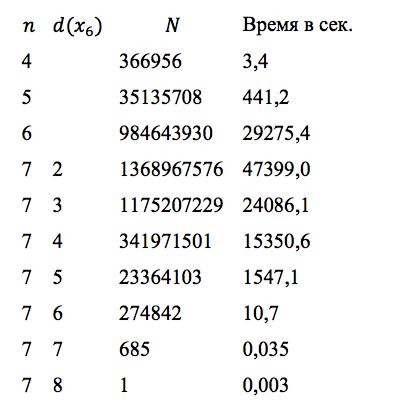
\includegraphics[width=0.4\textwidth]{AM/table1}
	%\caption{Табл. 1. Информация о длительности вычислений для пред-нормализованных  $(n,15-n)${}-графов порядка 15.}
\end{figure}
%\begin{flushleft}\label{AKM_ch1_tab1}
%\tablefirsthead{}
%\tablehead{}
%\tabletail{}
%\tablelasttail{}
%\begin{tabular}{|m{0.543cm}|m{1.375cm}|m{2.725cm}|m{2.799cm}|}\hline
% $n$ &
% $d(x_6)$ &
% $N$ &
%{\color[rgb]{0.5019608,0.5019608,0.5019608} Время в сек.}\\ \hline
%{\color[rgb]{0.5019608,0.5019608,0.5019608} 4} &
%~
% &
%{\selectlanguage{english}\color[rgb]{0.5019608,0.5019608,0.5019608} 366956} &
%{\color[rgb]{0.5019608,0.5019608,0.5019608} 3\foreignlanguage{english}{,}4}\\ \hline
%{\color[rgb]{0.5019608,0.5019608,0.5019608} 5} &
%~
% &
%{\color[rgb]{0.5019608,0.5019608,0.5019608} 35135708} &
%{\color[rgb]{0.5019608,0.5019608,0.5019608} 441\foreignlanguage{english}{,}2}\\ \hline
%{\color[rgb]{0.5019608,0.5019608,0.5019608} \foreignlanguage{english}{6}} &
%~
% &
%{\color[rgb]{0.5019608,0.5019608,0.5019608} 984643930} &
%{\color[rgb]{0.5019608,0.5019608,0.5019608} 29275\foreignlanguage{english}{,}4}\\ \hline
%{\color[rgb]{0.5019608,0.5019608,0.5019608} \foreignlanguage{english}{7}} &
%{\color[rgb]{0.5019608,0.5019608,0.5019608} \foreignlanguage{english}{2}} &
%{\color[rgb]{0.5019608,0.5019608,0.5019608} 1368967576} &
%{\color[rgb]{0.5019608,0.5019608,0.5019608} 47399\foreignlanguage{english}{,}0}\\ \hline
%{\color[rgb]{0.5019608,0.5019608,0.5019608} \foreignlanguage{english}{7}} &
%{\color[rgb]{0.5019608,0.5019608,0.5019608} \foreignlanguage{english}{3}} &
%{\color[rgb]{0.5019608,0.5019608,0.5019608} 1175207229} &
%{\color[rgb]{0.5019608,0.5019608,0.5019608} 24086\foreignlanguage{english}{,}1}\\ \hline
%{\color[rgb]{0.5019608,0.5019608,0.5019608} \foreignlanguage{english}{7}} &
%{\color[rgb]{0.5019608,0.5019608,0.5019608} \foreignlanguage{english}{4}} &
%{\color[rgb]{0.5019608,0.5019608,0.5019608} 341971501} &
%{\color[rgb]{0.5019608,0.5019608,0.5019608} 15350\foreignlanguage{english}{,}6}\\ \hline
%{\color[rgb]{0.5019608,0.5019608,0.5019608} 7} &
%{\color[rgb]{0.5019608,0.5019608,0.5019608} \foreignlanguage{english}{5}} &
%{\color[rgb]{0.5019608,0.5019608,0.5019608} 23364103} &
%{\color[rgb]{0.5019608,0.5019608,0.5019608} 1547\foreignlanguage{english}{,}1}\\ \hline
%{\color[rgb]{0.5019608,0.5019608,0.5019608} 7} &
%{\color[rgb]{0.5019608,0.5019608,0.5019608} \foreignlanguage{english}{6}} &
%{\color[rgb]{0.5019608,0.5019608,0.5019608} 274842} &
%{\color[rgb]{0.5019608,0.5019608,0.5019608} 10\foreignlanguage{english}{,}7}\\ \hline
%{\color[rgb]{0.5019608,0.5019608,0.5019608} 7} &
%{\color[rgb]{0.5019608,0.5019608,0.5019608} \foreignlanguage{english}{7}} &
%{\color[rgb]{0.5019608,0.5019608,0.5019608} 685} &
%{\color[rgb]{0.5019608,0.5019608,0.5019608} 0\foreignlanguage{english}{,}035}\\ \hline
%{\color[rgb]{0.5019608,0.5019608,0.5019608} 7} &
%{\color[rgb]{0.5019608,0.5019608,0.5019608} \foreignlanguage{english}{8}} &
%{\color[rgb]{0.5019608,0.5019608,0.5019608} 1} &
%{\color[rgb]{0.5019608,0.5019608,0.5019608} 0\foreignlanguage{english}{,}003 }\\ \hline
%\end{tabular}
%\end{flushleft}

\textbf{Информация о длительности вычислений. }Понятно, что в режиме вытесняющей мультизадачности длительность
вычислений носит условный характер и стремление к чрезмерной точности вычислений здесь неуместно. Тем не менее, мы
нашли допустимым записать в последней колонке таблицы \ref{AKM_ch1_tab1} длительности вычислений, измеренные в одном из компьютерных
экспериментов (временные параметры в других экспериментах несколько отличались от приведенных в таблице). Вычисления
для  $(n,15-n)${}-графов проводились отдельно для  $n=4,5,6$ \ и 7; при этом для  $n=7$ \ рассматривались семь случаев
в зависимости от степени вершины  $x_6$\ (см. второй столбец таблицы). Значение  $N$ \ в предпоследней колонке таблицы
- количество преднормализованных графов; количество нормализованных графов (для которых только и запускается жадный
алгоритм), соответствующих тому или иному конкретному случаю, существенно меньше.

%\section{Заключение}\label{AKM_ch1_7}
Предложенный в разделах \ref{AKM_ch2} и \ref{AKM_ch3} подход не только позволяет доказать, что все
$(n,15-n)${}-\textit{графы }интервально раскрашиваемы, но открывает перспективы и для проверки интервальной
раскрашиваемости двудольных графов большего порядка. Например, вычислительные эксперименты для  $(n,16-n)${}-графов
показали, что в случаях  $n=4,5$ \ и 6 все преднормализованные  $(n,16-n)${}-графы интервально раскрашиваемы, при этом
значения  $N$ \ и длительности вычислений равны соответственно: при  $n=4$: 767910 графов, 7,3 сек; при  $n=5$:
126091168 графов, 1993,0 сек; при  $n=6$: 6536939854 графов, 95178,2 сек.

Характеристики использованного авторами компьютерного обеспечения: \foreignlanguage{english}{Surface},
\foreignlanguage{english}{Windows} 10 \foreignlanguage{english}{Pro}, \foreignlanguage{english}{Processor}:
\foreignlanguage{english}{Intel}(\foreignlanguage{english}{R})
\foreignlanguage{english}{Core}(\foreignlanguage{english}{TM})
\foreignlanguage{english}{i}5-4300\foreignlanguage{english}{U} \foreignlanguage{english}{CPU} ©
1.90\foreignlanguage{english}{GHz} 2.50 \foreignlanguage{english}{GHz}, \foreignlanguage{english}{RAM}: 8.00
\foreignlanguage{english}{GB}, \foreignlanguage{english}{System} \foreignlanguage{english}{type}:
64-\foreignlanguage{english}{bit} \foreignlanguage{english}{Operating} \foreignlanguage{english}{System},
\foreignlanguage{english}{x}64-\foreignlanguage{english}{based}.

\begin{figure}[H]\label{AKM_ch1_img2}
	\centering
	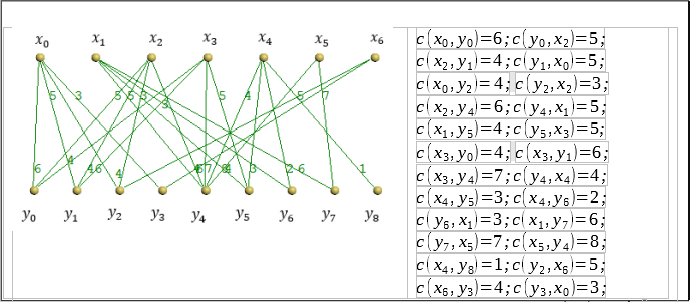
\includegraphics[width=1\textwidth]{AM/2}
	\caption{Пример вывода интервальной раскраски пред-нормализованного (7,9)-графа.}
\end{figure}

Разработанное программное обеспечение обладает некоторыми дополнительными функциями, непринципиальными для целей данного
сообщения. 
Среди них: различные формы представления графов и кусочно-непрерывных путей, графический и текстовый вывод интервальной
раскраски выбранного пользователем графа, в частности, преднормализованного. Пример такого вывода приведен на рис.\ref{AKM_ch1_img2}.






%%%%%%%%%%%%%%%%%%%%%%%%%%%
%%%%%%%%%%%%%%%%%%%%%%%%%%%
%%%%%%%%%%%%%%%%%%%%%%%%%%%





\chapter{Автоматизация создания тестовых заданий по языку программирования}\label{AKM_ch2}


\section{Компьютерное тестирование в образовании}\label{AKM_ch2_1}
Если вопросы целесообразности тотального компьютерного тестирования справедливо считаются в
преподавательской среде спорными, то роль тестов в качестве одного из инструментов обеспечения независимости и
объективности контроля усвоения учебного материала не вызывает сомнений. Важно и то, что наличие электронных средств
оценивания знаний студентов считается одним из необходимых условий для успешной аккредитации вуза. <<Ручная>> разработка
качественных и многочисленных тестовых единиц по каждой учебной дисциплине (в среднем по 500 тестовых единиц по каждой
дисциплине), причем --- в пяти формах (требование Управления качеством образования вуза), представляется практически
непосильным трудом, если, например, на кафедре всего восемь штатных преподавателей, а количество учебных дисциплин
превышает 60.
Цель данного раздела --- разработать схему для автоматизации процесса генерации тестовых материалов по языку
программирования.

\section{Типы тестовых заданий и программное обеспечение $А \rightarrow В$}\label{AKM_ch2_2}
2.2.1 Пять основных типов тестовых заданий:

1) выбор единственного правильного ответа из предложенного набора ответов;

2) выбор всех правильных ответов из предложенного набора ответов;

3) упорядочение элементов ответа в правильном порядке;

4) установление соответствия между элементами двух множеств;

5) самостоятельное вычисление ответа.

Примечание. Дополнительный, 6-й тип задания подразумевает исследование некоторой нестандартной ситуации.

2.2.2 Взаимосвязь двух программ

Сгенерированное нашим программным обеспечением (\foreignlanguage{english}{A}) тестовое задание предполагается в процессе
компьютерного тестирования отобразить на экране программой (\foreignlanguage{english}{B}), используемой вузовской
структурой тестирования, в виде, удобном для формулировки ответа в интерактивном режиме. Поэтому сформулированное
программой \foreignlanguage{english}{A} тестовое задание должно состоять из двух частей: первая отображается программой
В на экране для прочтения студентом, вторая используется для проверки правильности ответа студента. В следующих
примерах вторая часть выделена желтым цветом фона. Для локализации отдельного тестового задания среди других
(№Вопрос\foreignlanguage{english}{t}) и отдельных элементов ответа внутри тестового задания (№Да, №Нет) служит
специальный символ <<№>>. Заключительный для заголовка задания <<№Вопрос\foreignlanguage{english}{t}>> цифровой символ,
обозначенный здесь через <<\foreignlanguage{english}{t}>>, информирует студента о типе тестового задания (0, …, 5 или 6).


2.2.3 Иллюстрация на примерах - результатах программы А

\begin{example}\label{AKM_ch2_ex1}
	\
	
	\begin{figure}[H]
		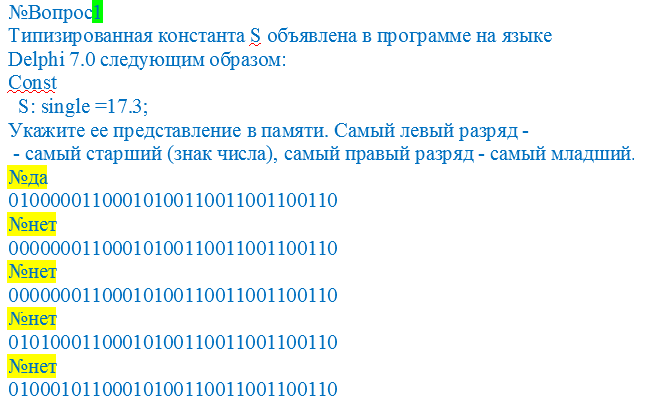
\includegraphics[width=0.7\textwidth]{AM/ex1_ch2}
		%\caption{Пример вывода интервальной раскраски пред-нормализованного (7,9)-графа.}
	\end{figure}
\end{example}
%Пример 1.
%
%\textcolor[rgb]{0.0,0.4392157,0.7529412}{№Вопрос1}
%
%\textcolor[rgb]{0.0,0.4392157,0.7529412}{Типизированная константа S объявлена в программе на языке }
%
%\foreignlanguage{english}{\textcolor[rgb]{0.0,0.4392157,0.7529412}{Delphi 7.0
%}}\textcolor[rgb]{0.0,0.4392157,0.7529412}{следующим}\foreignlanguage{english}{\textcolor[rgb]{0.0,0.4392157,0.7529412}{
%}}\textcolor[rgb]{0.0,0.4392157,0.7529412}{образом}\foreignlanguage{english}{\textcolor[rgb]{0.0,0.4392157,0.7529412}{:}}
%
%\foreignlanguage{english}{\textcolor[rgb]{0.0,0.4392157,0.7529412}{Const}}
%
%\foreignlanguage{english}{\textcolor[rgb]{0.0,0.4392157,0.7529412}{\ \ S: single =17.3;}}
%
%\textcolor[rgb]{0.0,0.4392157,0.7529412}{Укажите ее представление в памяти. Самый левый разряд - }
%
%\textcolor[rgb]{0.0,0.4392157,0.7529412}{\ {}- самый старший (знак числа), самый правый разряд - самый младший.}
%
%\textcolor[rgb]{0.0,0.4392157,0.7529412}{№да}
%
%\textcolor[rgb]{0.0,0.4392157,0.7529412}{01000001100010100110011001100110}
%
%\textcolor[rgb]{0.0,0.4392157,0.7529412}{№нет}
%
%\textcolor[rgb]{0.0,0.4392157,0.7529412}{00000001100010100110011001100110}
%
%\textcolor[rgb]{0.0,0.4392157,0.7529412}{№нет}
%
%\textcolor[rgb]{0.0,0.4392157,0.7529412}{00000001100010100110011001100110}
%
%\textcolor[rgb]{0.0,0.4392157,0.7529412}{№нет}
%
%\textcolor[rgb]{0.0,0.4392157,0.7529412}{01010001100010100110011001100110}
%
%\textcolor[rgb]{0.0,0.4392157,0.7529412}{№нет}
%
%\textcolor[rgb]{0.0,0.4392157,0.7529412}{01000101100010100110011001100110}

\begin{example}\label{AKM_ch2_ex2}
	\

	\begin{figure}[H]
		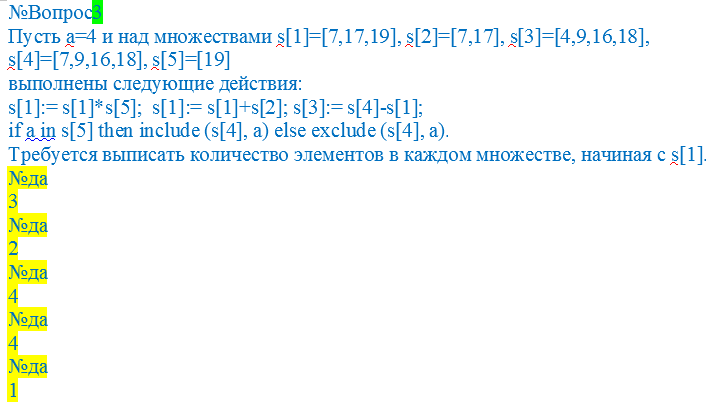
\includegraphics[width=0.8\textwidth]{AM/ex2_ch2}
		%\caption{Пример вывода интервальной раскраски пред-нормализованного (7,9)-графа.}
	\end{figure}
\end{example}

%\textcolor{black}{Пример 2.}
%
%\textcolor[rgb]{0.0,0.4392157,0.7529412}{№Вопрос3}
%
%\textcolor[rgb]{0.0,0.4392157,0.7529412}{Пусть a=4 и над множествами s[1]=[7,17,19], s[2]=[7,17], s[3]=[4,9,16,18],
%	s[4]=[7,9,16,18], s[5]=[19] }
%
%\textcolor[rgb]{0.0,0.4392157,0.7529412}{выполнены}\foreignlanguage{english}{\textcolor[rgb]{0.0,0.4392157,0.7529412}{
%}}\textcolor[rgb]{0.0,0.4392157,0.7529412}{следующие}\foreignlanguage{english}{\textcolor[rgb]{0.0,0.4392157,0.7529412}{
%}}\textcolor[rgb]{0.0,0.4392157,0.7529412}{действия}\foreignlanguage{english}{\textcolor[rgb]{0.0,0.4392157,0.7529412}{:}}
%
%\foreignlanguage{english}{\textcolor[rgb]{0.0,0.4392157,0.7529412}{s[1]:= s[1]*s[5]; \ s[1]:= s[1]+s[2]; s[3]:=
%		s[4]-s[1];}}
%
%\foreignlanguage{english}{\textcolor[rgb]{0.0,0.4392157,0.7529412}{if a in s[5] then include (s[4], a) else exclude
%		(s[4], a).}}
%
%\textcolor[rgb]{0.0,0.4392157,0.7529412}{Требуется выписать количество элементов в каждом множестве, начиная с s[1].}
%
%\textcolor[rgb]{0.0,0.4392157,0.7529412}{№да}
%
%\textcolor[rgb]{0.0,0.4392157,0.7529412}{3}
%
%\textcolor[rgb]{0.0,0.4392157,0.7529412}{№да}
%
%\textcolor[rgb]{0.0,0.4392157,0.7529412}{2}
%
%\textcolor[rgb]{0.0,0.4392157,0.7529412}{№да}
%
%\textcolor[rgb]{0.0,0.4392157,0.7529412}{4}
%
%\textcolor[rgb]{0.0,0.4392157,0.7529412}{№да}
%
%\textcolor[rgb]{0.0,0.4392157,0.7529412}{4}
%
%\textcolor[rgb]{0.0,0.4392157,0.7529412}{№да}
%
%\textcolor[rgb]{0.0,0.4392157,0.7529412}{1}

\begin{example}\label{AKM_ch2_ex3}
	\
	
	\begin{figure}[H]
		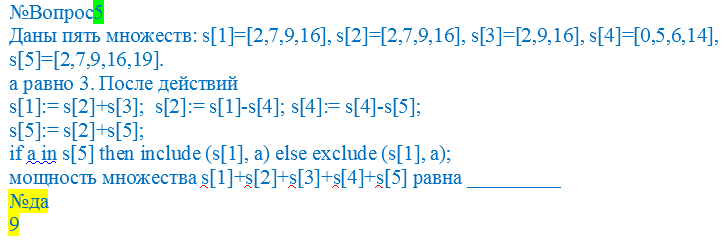
\includegraphics[width=0.8\textwidth]{AM/ex3_ch2}
		%\caption{Пример вывода интервальной раскраски пред-нормализованного (7,9)-графа.}
	\end{figure}
\end{example}

%\textcolor{black}{Пример 3.}
%
%\textcolor[rgb]{0.0,0.4392157,0.7529412}{№Вопрос5}
%
%\textcolor[rgb]{0.0,0.4392157,0.7529412}{Даны пять множеств:
%}\foreignlanguage{english}{\textcolor[rgb]{0.0,0.4392157,0.7529412}{s}}\textcolor[rgb]{0.0,0.4392157,0.7529412}{[1]=[2,7,9,16],
%}\foreignlanguage{english}{\textcolor[rgb]{0.0,0.4392157,0.7529412}{s}}\textcolor[rgb]{0.0,0.4392157,0.7529412}{[2]=[2,7,9,16],
%}\foreignlanguage{english}{\textcolor[rgb]{0.0,0.4392157,0.7529412}{s}}\textcolor[rgb]{0.0,0.4392157,0.7529412}{[3]=[2,9,16],
%}\foreignlanguage{english}{\textcolor[rgb]{0.0,0.4392157,0.7529412}{s}}\textcolor[rgb]{0.0,0.4392157,0.7529412}{[4]=[0,5,6,14],
%}\foreignlanguage{english}{\textcolor[rgb]{0.0,0.4392157,0.7529412}{s}}\textcolor[rgb]{0.0,0.4392157,0.7529412}{[5]=[2,7,9,16,19].
%}
%
%\foreignlanguage{english}{\textcolor[rgb]{0.0,0.4392157,0.7529412}{a
%}}\textcolor[rgb]{0.0,0.4392157,0.7529412}{равно}\foreignlanguage{english}{\textcolor[rgb]{0.0,0.4392157,0.7529412}{ 3.
%}}\textcolor[rgb]{0.0,0.4392157,0.7529412}{После}\foreignlanguage{english}{\textcolor[rgb]{0.0,0.4392157,0.7529412}{
%}}\textcolor[rgb]{0.0,0.4392157,0.7529412}{действий}\foreignlanguage{english}{\textcolor[rgb]{0.0,0.4392157,0.7529412}{
%}}
%
%\foreignlanguage{english}{\textcolor[rgb]{0.0,0.4392157,0.7529412}{s[1]:= s[2]+s[3]; \ s[2]:= s[1]-s[4]; s[4]:=
%		s[4]-s[5];}}
%
%\foreignlanguage{english}{\textcolor[rgb]{0.0,0.4392157,0.7529412}{s[5]:= s[2]+s[5];}}
%
%\foreignlanguage{english}{\textcolor[rgb]{0.0,0.4392157,0.7529412}{if a in s[5] then include (s[1], a) else exclude
%		(s[1], a); }}
%
%\textcolor[rgb]{0.0,0.4392157,0.7529412}{мощность множества s[1]+s[2]+s[3]+s[4]+s[5] равна \_\_\_\_\_\_\_\_\_}
%
%\textcolor[rgb]{0.0,0.4392157,0.7529412}{№да}
%
%\textcolor[rgb]{0.0,0.4392157,0.7529412}{9}
%
%
%\bigskip

2.2.4 Ключевые слова в синтаксисе тестовых заданий - требование программы В

В заданиях типа 1, 2 и 5 ключевое слово №Да указывает программе \foreignlanguage{english}{B} на правильные элементы
ответа. В заданиях типа 3 и 4 ожидаемая от испытуемого правильная последовательность элементов ответа сообщается
программе В последовательностью этих элементов в сгенерированном программой А задании, программа же В запоминает эту
последовательность, но выводит эти элементы на экран в перемешанном виде; в данном случае ключевое слово №Да не
является указателем на правильные элементы, оно играет лишь роль разделителя элементов ответа.

\section{Схема автоматизации процесса создания тестовых заданий}\label{AKM_ch2_3}
\hypertarget{Toc503377133}{}2.3.1 Сокращенная схема автоматизации

Продемонстрируем идею автоматизации генерации тестовых заданий на примере \ref{AKM_ch2_ex1}, соответствующему первому типу, обладающему
простейшей структурой по сравнению с другими типами. Как составить процедуру, генерирующую, скажем,
\foreignlanguage{english}{n}=1000 таких примеров?

Сначала следует создать \foreignlanguage{english}{n} попарно различных случайных чисел
\foreignlanguage{english}{s}[\foreignlanguage{english}{i}] типа \foreignlanguage{english}{Single},

после чего найти для каждого \foreignlanguage{english}{s}[\foreignlanguage{english}{i}] его 32-битное представление
\foreignlanguage{english}{b}0[\foreignlanguage{english}{i}] - <<единственный правильный ответ>> и произвольные четыре
32-битные последовательности \foreignlanguage{english}{b}1[\foreignlanguage{english}{i}],
\foreignlanguage{english}{b}2[\foreignlanguage{english}{i}], \foreignlanguage{english}{b}3[3],
\foreignlanguage{english}{b}4[\foreignlanguage{english}{i}], отличные друг от друга и от
\foreignlanguage{english}{b}0[\foreignlanguage{english}{i}], - <<четыре неправильных ответа>>,

в завершение сконструировать текст, отличающийся от текста примера 1 лишь заменой приведенного в примере числа 17.3 на
значение \foreignlanguage{english}{s}[\foreignlanguage{english}{i}], первого элемента ответа (после <<№да>>) - на
\foreignlanguage{english}{b}0[\foreignlanguage{english}{i}], остальных элементов ответа (после ключевого слова <<№нет>>)
- на \foreignlanguage{english}{b}1[\foreignlanguage{english}{i}],
\foreignlanguage{english}{b}2[\foreignlanguage{english}{i}], \foreignlanguage{english}{b}3[3],
\foreignlanguage{english}{b}4[\foreignlanguage{english}{i}] соответственно.

Таким образом, для всех \foreignlanguage{english}{n} тестовых заданий, являющихся вариациями примера 1, разъяснительный
текст является постоянным (назовем его <<текстовым шаблоном>>). Но в перечне тестовых заданий, из которых программа В
скомпонует полный тест, предлагаемый конкретному студенту, все текстовые шаблоны уникальны. С учетом того, что по
каждой учебной дисциплине предполагается около 20 различных тем, \foreignlanguage{english}{i}=1, …, 20, а по каждой
теме формулируются тестовые задания 5-6 типов, \foreignlanguage{english}{j}=1, …, 5 или 6 (тестовое задание
\foreignlanguage{english}{j}{}-го типа по \foreignlanguage{english}{i}{}-й теме назовем
<<\foreignlanguage{english}{i},\foreignlanguage{english}{j}{}-термом>>), то всего текстовых шаблонов получится больше
одной сотни.

2.3.2 Развернутая схема автоматизации создания i,j-терма

\foreignlanguage{english}{I}. В первой части программного кода для генерации
\foreignlanguage{english}{i},\foreignlanguage{english}{j}{}-терма объявляются и инициализируются основные объекты
(главным образом - тех типов, которые изучаются в \foreignlanguage{english}{i}{}-й теме), а также вспомогательные
переменные, среди которых, в частности, могут присутствовать переменные строкового типа, предназначенные для
запоминания результатов.

Инициализация производится в виде присвоения одиночных констант (например, 8, ‘\foreignlanguage{english}{A}’,
\foreignlanguage{english}{FALSE}, []) или константных выражений (например, \foreignlanguage{english}{not} 7,
\foreignlanguage{english}{trunc}(-6.5), ‘\foreignlanguage{english}{A}’+’\foreignlanguage{english}{B}’,
\foreignlanguage{english}{random} (2)).

Приведенные ниже примеры соответствуют случаю генерации 15,3-терма (тема 15 - <<Множества>>, тип 3 - <<Упорядоченное
перечисление элементов ответов>>).

{\centering
	\foreignlanguage{english}{1.1. }Раздел\foreignlanguage{english}{ }объявления\foreignlanguage{english}{
	}объектов\foreignlanguage{english}{:}
	\par}

	\begin{figure}[H]
		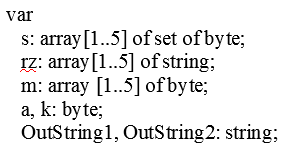
\includegraphics[width=0.3\textwidth]{AM/code1}
		%\caption{Пример вывода интервальной раскраски пред-нормализованного (7,9)-графа.}
	\end{figure}

%\foreignlanguage{english}{var}
%
%\foreignlanguage{english}{\ \ \ s: array[1..5] of set of byte;}
%
%\foreignlanguage{english}{\ \ \ rz: array[1..5] of string;}
%
%\foreignlanguage{english}{\ \ \ m: array [1..5] of byte;}
%
%\foreignlanguage{english}{\ \ \ a, k: byte;}
%
%\foreignlanguage{english}{\ \ \ OutString1, OutString2: string; \ }

{\centering
	1.2. Инициализация объектов:
	\par}

	\begin{figure}[H]
		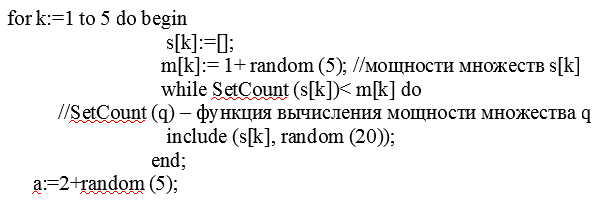
\includegraphics[width=0.7\textwidth]{AM/code2}
		%\caption{Пример вывода интервальной раскраски пред-нормализованного (7,9)-графа.}
	\end{figure}

%\foreignlanguage{english}{for} \foreignlanguage{english}{k}:=1 \foreignlanguage{english}{to} 5
%\foreignlanguage{english}{do} \foreignlanguage{english}{begin}
%
%\ \ \ \ \ \ \ \ \ \ \ \ \ \ \ \ \ \ \ \ \ \ \ \ \ \ \ \ \ \ \ \foreignlanguage{english}{s}[\foreignlanguage{english}{k}]:=[];
%
%\ \ \ \ \ \ \ \ \ \ \ \ \ \ \ \ \ \ \ \ \ \ \ \ \ \ \ \ \ \ \foreignlanguage{english}{m}[\foreignlanguage{english}{k}]:=
%1+ \foreignlanguage{english}{random} (5); //мощности множеств
%\foreignlanguage{english}{s}[\foreignlanguage{english}{k}]
%
%\ \ \ \ \ \ \ \ \ \ \ \ \ \ \ \ \ \ \ \ \ \ \ \ \ \ \ \ \ \ \foreignlanguage{english}{while SetCount (s[k]){\textless}
%	m[k] do}
%
%\foreignlanguage{english}{\ \ \ \ \ \ \ \ \ \ }//\foreignlanguage{english}{SetCount} (\foreignlanguage{english}{q}) -
%функция вычисления мощности множества \foreignlanguage{english}{q}
%
%\ \ \ \ \ \ \ \ \ \ \ \ \ \ \ \ \ \ \ \ \ \ \ \ \ \ \ \ \ \ \ \foreignlanguage{english}{include (s[k], random (20));}
%
%\foreignlanguage{english}{\ \ \ \ \ \ \ \ \ \ \ \ \ \ \ \ \ \ \ \ \ \ \ \ \ \ \ \ end;}
%
%\foreignlanguage{english}{\ \ \ \ \ }a:=2+random (5);
%
%
%\bigskip

Затем над объектами выполняются действия, проверка понимания которых составляет цель опроса по данному
\foreignlanguage{english}{i},\foreignlanguage{english}{j}{}-терму. Результаты таких действий запоминаются в строковом
формате.

{\centering
	1.3. Блок действий:
	\par}

	\begin{figure}[H]
		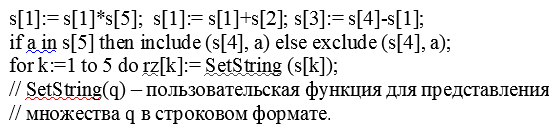
\includegraphics[width=0.6\textwidth]{AM/code3}
		%\caption{Пример вывода интервальной раскраски пред-нормализованного (7,9)-графа.}
	\end{figure}

%\foreignlanguage{english}{s}[1]:= \foreignlanguage{english}{s}[1]*\foreignlanguage{english}{s}[5];
%\ \foreignlanguage{english}{s}[1]:= \foreignlanguage{english}{s}[1]+\foreignlanguage{english}{s}[2];
%\foreignlanguage{english}{s}[3]:= \foreignlanguage{english}{s}[4]-\foreignlanguage{english}{s}[1];
%
%\foreignlanguage{english}{if a in s[5] then include (s[4], a) else exclude (s[4], a);}
%
%\foreignlanguage{english}{for k:=1 to 5 do rz[k]:= SetString (s[k]);}
%
%// \foreignlanguage{english}{SetString}(\foreignlanguage{english}{q}) - пользовательская функция для представления
%
%// множества \foreignlanguage{english}{q} в строковом формате.
%
%
%\bigskip

\foreignlanguage{english}{II}. Во второй части программного кода
\foreignlanguage{english}{i},\foreignlanguage{english}{j}{}-терма формируются две текстовые величины: открытая часть
OutString1, непосредственно предъявляемая испытуемому, и скрытая часть OutString2, предъявляемая испытуемому лишь после
обработки программным обеспечением \foreignlanguage{english}{B}.

{\centering
	2.1. Формирование OutString1:
	\par}

\begin{figure}[H]
	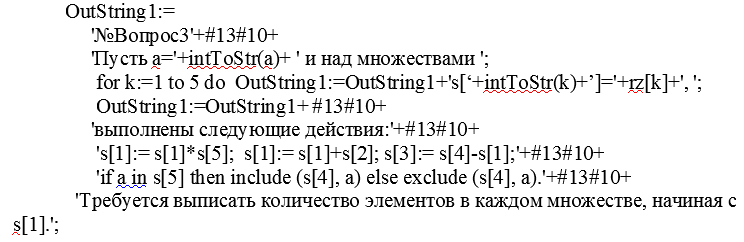
\includegraphics[width=0.8\textwidth]{AM/code4}
	%\caption{Пример вывода интервальной раскраски пред-нормализованного (7,9)-графа.}
\end{figure}

%OutString1:=
%
%\ \ \ \ \ {}'№Вопрос3'+\#13\#10+
%
%\ \ \ \ \ {}'Пусть a='+intToStr(a)+ ' и над множествами ';
%
%\ \ \ \ \ \ \foreignlanguage{english}{for k:=1 to 5 do \ OutString1:=OutString1+'s[‘+intToStr(k)+’]='+rz[k]+', ';}
%
%\foreignlanguage{english}{\ \ \ \ \ \ }OutString1:=OutString1+ \#13\#10+
%
%\ \ \ \ \ {}'выполнены следующие действия:'+\#13\#10+
%
%\ \ \ \ \ \ \foreignlanguage{english}{{}'s[1]:= s[1]*s[5]; \ s[1]:= s[1]+s[2]; s[3]:= s[4]-s[1];'+\#13\#10+}
%
%\foreignlanguage{english}{\ \ \ \ \ \ {}'if a in s[5] then include (s[4], a) else exclude (s[4], a).'+\#13\#10+}
%
%\foreignlanguage{english}{\ \ }{}'Требуется выписать количество элементов в каждом множестве, начиная с s[1].';

{\centering
	\foreignlanguage{english}{2.2. }Формирование\foreignlanguage{english}{ OutString2:}
	\par}

\begin{figure}[H]
	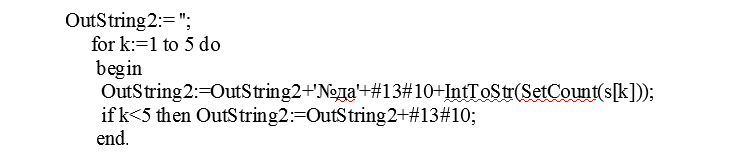
\includegraphics[width=0.8\textwidth]{AM/code5}
	%\caption{Пример вывода интервальной раскраски пред-нормализованного (7,9)-графа.}
\end{figure}

%\foreignlanguage{english}{OutString2:= '{}';}
%
%\foreignlanguage{english}{\ \ \ \ \ for k:=1 to 5 do}
%
%\foreignlanguage{english}{\ \ \ \ \ \ begin}
%
%%atansion!
%%\foreignlanguage{english}{\ \ \ \ \ \ \ OutString2:=OutString2+'№ да'+\#13\#10+IntToStr(SetCount(s[k]));}
%%\foreignlanguage{english}{\ \ \ \ \ \ \ OutString2:=OutString2+'#да'+\#13\#10+IntToStr(SetCount(s[k]));}
%
%\foreignlanguage{english}{\ \ \ \ \ \ \ if k{\textless}5 then OutString2:=OutString2+\#13\#10;}
%
%\foreignlanguage{english}{\ \ \ \ \ \ end}.
%
%
%\bigskip

В конце второй части осуществляется вывод обоих текстов в файл, соответствующий \textit{модулю}, - относительно
самодостаточной совокупности из нескольких тем, включая и рассматриваемую \foreignlanguage{english}{i}{}-ю тему.

2-й из приведенных выше примеров получен описанной процедурой, примеры 1 и 3 - иными процедурами, но с аналогичной
структурой.

\section{Нестандартные ситуации для заданий дополнительного типа}\label{AKM_ch2_4}
\hypertarget{Toc503377134}{}Независимо от способа составления, задания 6-го типа должны проверяться преподавателем
традиционным способом.

Приведем несколько нестандартных ситуаций в качестве материала для составления заданий 6-го типа.

2.4.1 Константное выражение

Вопрос. Что напечатают программы А и В (они различаются лишь символами, выделенными красным цветом)?
\begin{figure}[H]
	\centering
	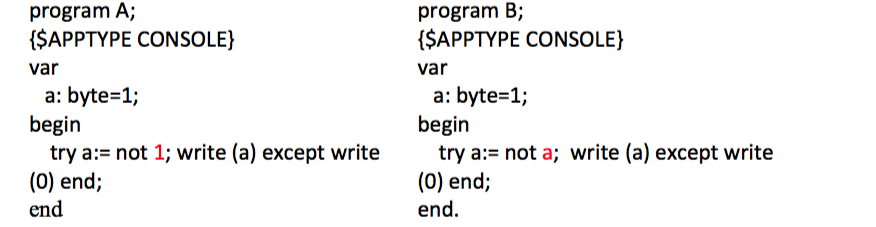
\includegraphics[width=0.9\textwidth]{AM/table2}
	%\caption{Табл. 1. Информация о длительности вычислений для пред-нормализованных  $(n,15-n)${}-графов порядка 15.}
\end{figure}
%\begin{flushleft}
%\tablefirsthead{}
%\tablehead{}
%\tabletail{}
%\tablelasttail{}
%\begin{supertabular}{m{8.0390005cm}m{8.304cm}}
%\foreignlanguage{english}{program }А\foreignlanguage{english}{;}
%
%\foreignlanguage{english}{\{\$APPTYPE CONSOLE\}}
%
%\foreignlanguage{english}{var}
%
%\foreignlanguage{english}{\ \ \ a: byte=1;}
%
%\foreignlanguage{english}{begin}
%
%\foreignlanguage{english}{\ \ \ \ try a:= not }\foreignlanguage{english}{\textcolor{red}{1}}\foreignlanguage{english}{;
%write (a) except write (0) end;}
%
%\foreignlanguage{english}{end} &
%\foreignlanguage{english}{program }В\foreignlanguage{english}{;}
%
%\foreignlanguage{english}{\{\$APPTYPE CONSOLE\} }
%
%\foreignlanguage{english}{var}
%
%\foreignlanguage{english}{\ \ \ a: byte=1; }
%
%\foreignlanguage{english}{begin}
%
%\foreignlanguage{english}{\ \ \ \ try a:= not }\foreignlanguage{english}{\textcolor{red}{a}}\foreignlanguage{english}{;
%\ write (a) except write (0) end;}
%
%end.\\
%\end{supertabular}
%\end{flushleft}

\bigskip

Ответ. А - ничего (ошибка компиляции), В - 254.

2.4.2 Переполнение

Вопрос. Чему равны значения типизированных констант \foreignlanguage{english}{correct} и
\foreignlanguage{english}{error}?

\begin{figure}[H]
	\centering
	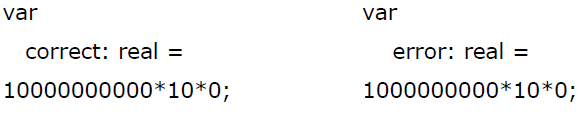
\includegraphics[width=0.7\textwidth]{AM/code6}
	%\caption{Табл. 1. Информация о длительности вычислений для пред-нормализованных  $(n,15-n)${}-графов порядка 15.}
\end{figure}

%\begin{flushleft}
%\tablefirsthead{}
%\tablehead{}
%\tabletail{}
%\tablelasttail{}
%\begin{supertabular}{m{8.041cm}m{8.041cm}}
%{\color[rgb]{0.5019608,0.5019608,0.5019608} \foreignlanguage{english}{var}}
%
%{\color[rgb]{0.5019608,0.5019608,0.5019608} \foreignlanguage{english}{\ \ \ correct: real = 10000000000*10*0;}} &
%{\color[rgb]{0.5019608,0.5019608,0.5019608} \foreignlanguage{english}{var}}
%
%{\color[rgb]{0.5019608,0.5019608,0.5019608} \foreignlanguage{english}{\ \ \ \ error: real = 1000000000*10*0;}}\\
%\end{supertabular}
%\end{flushleft}

Ответ: \foreignlanguage{english}{correct} равно нулю, при вычислении второго выражения (для
\foreignlanguage{english}{error}) - ошибка компиляции.

2.4.3 Неявное преобразование к типу extended

Вопрос. Какое значение напечатает программа:

\begin{figure}[H]
	\centering
	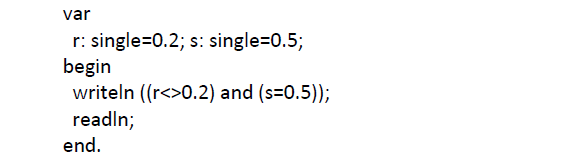
\includegraphics[width=0.7\textwidth]{AM/code7}
	%\caption{Табл. 1. Информация о длительности вычислений для пред-нормализованных  $(n,15-n)${}-графов порядка 15.}
\end{figure}
%\foreignlanguage{english}{var}
%
%\ \ \foreignlanguage{english}{r}: \foreignlanguage{english}{single}=0.2; \foreignlanguage{english}{s}:
%\foreignlanguage{english}{single}=0.5;
%
%\foreignlanguage{english}{begin}
%
%\foreignlanguage{english}{\ \ writeln ((r{\textless}{\textgreater}0.2) and (s=0.5));}
%
%\foreignlanguage{english}{\ \ }readln;
%
%end.

Ответ: \foreignlanguage{english}{TRUE}.

%\section{Заключение}\label{AKM_ch2_5}
Изложенная схема легла в основу программного обеспечения для компьютерной генерации тестовых пунктов по языку программирования Delphi 7.0. Разработанные тесты прошла экспертизу специалистов Управления качеством образования ФГБОУ <<Дагестанский государственный университет>>. Соответствующая статья отправлена в редакцию Международного научно-исследовательского журнала, материалы на получение свидетельства на Программу для ЭВМ отправлена в Роспатент, подана заявка на участие студента ФМиКН ДГУ Гаджимирзаева Ш.М. в работе Всероссийской конференции в марте 2018 г.














%%%%%%%%%%%%%%%%%%%%%%%%%%%
%%%%%%%%%%%%%%%%%%%%%%%%%%%
%%%%%%%%%%%%%%%%%%%%%%%%%%%






\chapter{Алгоритм компьютерного сопровождения некоторых задач распределения учебной нагрузки}\label{AKM_ch3}

\section{Постановка задачи}\label{AKM_ch3_1}
%Распределение учебной нагрузки вузовской кафедры практически никогда не начинается <<с
%чистого листа>>. В качестве исходного, <<чернового>> выступает распределение, унаследованное от предыдущего учебного года.
%С другой стороны, <<черновое>> распределение никогда не может быть принято за <<беловик>> без дополнительной работы над
%ошибками (изменяется количество студентов в учебных группах, ежегодно изменяется состав актуальных учебных дисциплин
%категории <<по выбору>>, в рамках оптимизации учебных нагрузок в связи с финансовыми проблемами вуза могут быть
%скорректированы объемы учебных часов).

К распространенным формам представления учебных нагрузок, утвержденных кафедре учебно-методическим управлением вуза
(далее кратко --- <<план кафедры>>), и индивидуальных учебных нагрузок, планируемых руководителем кафедры отдельным
преподавателям (далее --- <<индивидуальные планы>>), является отведение этим <<планам>> отдельных листов рабочей книги MS
Excel со строго продуманной структурой.

Предполагается, что исходные данные программы представлены рабочей книгой \foreignlanguage{english}{Excel}, где рабочие
листы содержат индивидуальные учебные нагрузки преподавателей кафедры на учебный год; в начальной ячейке
$i$-го листа $(i=1,2, \ldots, n)$ --- указана
основная категория преподавателя (штатный, работодатель, совместитель или <<специальный>>), преподаватели разных
категорий образуют непересекающиеся множества; на пересечении со столбцами 10, …, 30 каждой
\foreignlanguage{english}{j}{}-й строки из диапазона 3-20 (27-44) \foreignlanguage{english}{i}{}-й лист содержит число
часов, запланированных \foreignlanguage{english}{i}{}-му преподавателю в семестре 1 (семестре 2) в той учебной группе и
по той учебной дисциплине, сведения о которых указаны в начальных ячейках \foreignlanguage{english}{j}{}-й строки; при
этом множество преподавателей <<дополнительной>> категории, выполняющих часть учебной нагрузки на почасовой оплате, может
иметь непустое пересечение с любым из упомянутых четырех множеств, соответствующая учебная нагрузка задается в строках
21-24 или 45-49 в зависимости от семестра.

Количество рабочих ячеек обычно достаточно велико, например, их количество даже в плане сравнительно компактной кафедры
ДМиИ достигает 150*20 = 3000. Поэтому искомое распределение требует последовательное выполнение целого ряда итераций.

\section{Основные функции программного комплекса}\label{AKM_ch3_2}

Руководитель кафедры должен распределить учебную нагрузку кафедры с учетом: 
\begin{enumerate}[a)]
  \item квалификации и специализации преподавателей,
  \item соотношений <<должность>> -- <<объем часов>>,  
  \item преемственности нагрузок, 
  \item приемлемого соотношения часов каждого типа: <<лекционные>> -- <<практические>> -- <<лабораторные>> -- <<научное руководство выпускными квалификационными работами>> - и т.д. внутри выделенного преподавателю объема часов.
\end{enumerate}
 

Распределение учебных нагрузок кафедры должна получить логическое завершение в виде создания сводных таблиц
распределения для представления в учебно-методическое управление вуза. Предусмотрено построение трех сводных таблиц
распределения учебных нагрузок (промежуточные - для каждого из двух семестров и итоговая - за год). Каждая таблица
формируется на отдельном листе рабочей книги \foreignlanguage{english}{Excel} с разбиением на подтаблицы,
соответствующие преподавателям каждой из пяти категорий (четырем основным и одной <<дополнительной>>). При этом итоговая
таблица имеет развернутый вид - с учетом каждого типа учебной нагрузки (лекции, зачеты, курсовые, преддипломная
практика и т.п.), а промежуточные таблицы выводятся в сжатом виде - для каждого преподавателя каждой из пяти подтаблиц
указываются лишь суммарные часы и часы по лекционному, семинарскому и лабораторному типу занятий; такие требования
обычно предъявляются учебно-методическими управлениями вузов.

В течение всего итерационного процесса распределения нагрузок необходимо обеспечивать корректность представления
информации во всех индивидуальных планах преподавателей: они не должны содержать пункты, оставшиеся от прошлогоднего
плана кафедры, но отсутствующие в текущем плане кафедры, информация в контрольных строках и контрольном столбце должна
действительно соответствовать соответствующим суммам.

Разработанная программа выполняет проверку правильности подведения итогов: а) по каждой учебной дисциплине, б) по
каждому виду занятий, в) по каждому типу оплаты (штатная, почасовая), г) по каждому семестру и за учебный год в целом.

\begin{figure}[H]
	\centering
	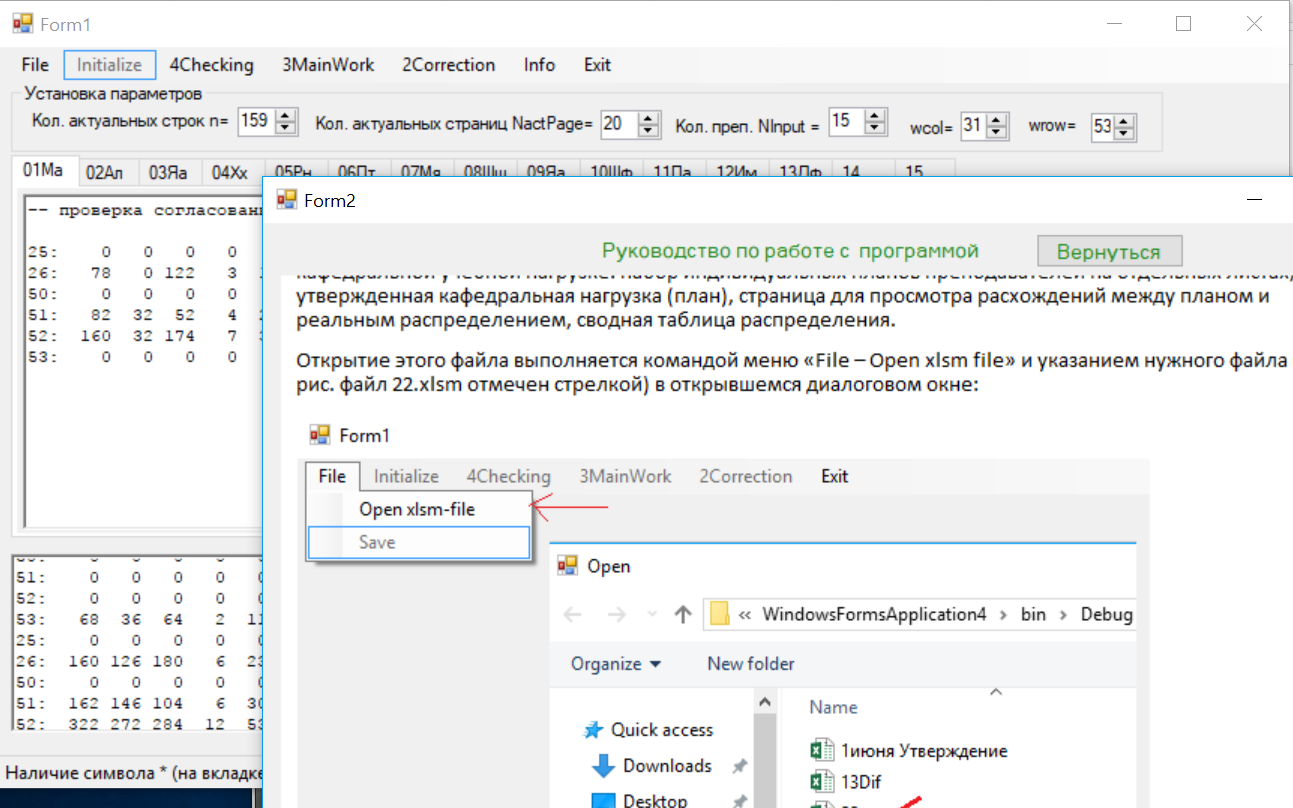
\includegraphics[width=1\textwidth]{AM/3}
	\caption{Запуск программы. Видны меню и электронный блокнот. В правой-нижней части отображается текст файла помощи
		(результат выбора команды меню \foreignlanguage{english}{Info}).}
\end{figure}

Программа способна успешно завершить начатый процесс распределения учебных нагрузок кафедры с частично заполненными
индивидуальными планами преподавателей и содержать следующие пункты в качестве обязательных: внутреннее согласование
индивидуальных планов, актуализация контингента учебных групп, ликвидация фантомных пунктов и устранение блужданий по
семестрам, вычисление и визуализация невязок, автоматизированное устранение малых невязок, персонификация
распределения, автоматическая верстка исходных данных к факультетскому расписанию, создание сводных таблиц
распределения.

В качестве программистского результата разработан проект на языке C\# с развитым и интуитивно понятым интерфейсом: меню
и панель быстрых инструментов, строка статуса и всплывающие подсказки, визуальные компоненты и подробное руководство к
использованию.

Завершенные в общих чертах стадии технологического процесса разработки программы: формулировка основных функций
программы и их решение (алгоритмы и воплощение в классах C\#), планирование и реализация интерфейса.


\bigskip

\section{Научная новизна и особенности проекта}\label{AKM_ch3_3}
Данный проект, разработанный на языке C\# в среде Visual Studio, имеет неоспоримые
предпочтения по сравнению с VBA-проектами и целым рядом рекламируемых в сети Интернет системами (часто реализованных
средствами 1C) не только по быстродействию или в плане интерфейса, но и по качеству реализации непростых
алгоритмических идей (так, развитые средства C\# для действий со строками послужили мотивацией к идее подготовки данных
к расписанию на основе описанной выше персонификации распределения, а простота реализации визуальных компонентов - к
идее использования электронного блокнота для отображения коллизий согласования индивидуальных планов).

%\section{Заключение}\label{AKM_ch3_4}
Практически все решения данного проекта являются новыми по сравнению со всеми известными
аналогичными системами:

{}- алгоритмы выявления в индивидуальных планах преподавателей фантомных и блуждающих учебных поручений;

{}- вычисление невязок и идея автоматизированного устранения невязок с малозначащими величинами (последняя еще не
воплощена в программе);

{}- персонификация распределения и алгоритм форматирования полученной персонификации для представления данных к учебному
расписанию факультета.

Подчеркнем, что ни одна из известных систем автоматизированного распределения учебных нагрузок не рассчитана собственно
на продолжение процесса распределения, исходя из уже существующего, унаследованного от предыдущего учебного года
распределения; аналогичным недостатком страдали и системы, использовавшиеся ранее (в течение более 10 лет) на кафедре
ДМиИ ДГУ. Многочисленные обсуждения с разработчиками кафедры ДМиИ ряда спорных вопросов помогли создать систему,
сильные стороны которой в наибольшей степени проявляются именно в той ситуации, которая наиболее часто встречается в
вузовской практике, а именно - когда распределение учебной нагрузки кафедры проводится в режиме исправления коллизий в
уже существующем распределении.

Программу рекомендуется использовать в работе лаборанта и заведующего вузовской кафедры и для автоматизации процесса
подготовки для учебно-методического управления вуза электронной документации о распределении учебных нагрузок кафедры.

Выполненная в данном направлении работа магистранта ФМиКН ДГУ Ибрагимовой З.И. представлена на конкурс <<Умник>> (в
настоящее время известно, что работа вышла в финал). Получены два свидетельства Роспатента для программы для ЭВМ \cite{AKM_ch3_bib1} - \cite{AKM_ch3_bib2}.












%%%%%%%%%%%%%%%%%%%%%%%%%%%
%%%%%%%%%%%%%%%%%%%%%%%%%%%
%%%%%%%%%%%%%%%%%%%%%%%%%%%





\chapter{Алгоритмическое и программное обеспечение для конкурсов и олимпиад}\label{AKM_ch4}


%
%\section{Введение}\label{AKM_ch4_1}
%Для таких вузовских структур, которые сочетают исследовательскую
%	деятельность с преподаванием дисциплин компьютерных направлений, естественным является сочетание учебно-методической
%	работы (в частности, издание учебных пособий с решениями нестандартных задач) с работой по подготовке студентов к
%	конкурсам и олимпиадам по программированию.

\section{Межрегиональная дистанционная олимпиада по программированию среди команд вузов СКФО}\label{AKM_ch4_2}

21 апреля 2017 г. в ФГБОУ ВО <<Дагестанский государственный университет>> под руководством Магомедова
	А.М. (составитель заданий и председатель жюри) состоялась вторая межрегиональная дистанционная олимпиада по
	программированию среди команд вузов СКФО. В олимпиаде приняли участие 37 команд.

В пособие \cite{AKM_ch4_bib1} вошли формулировки заданий, обсуждение их решений и листинги программ на языке C\#, а
	также информация о результатах команд.

\section{Алгоритмическое обеспечение конкурсов по 3D-моделированию}\label{AKM_ch4_3}

\textcolor{black}{Около 40 упражнений по 3ds Max с решениями вошли в изданное в 2017 г. пособие \cite{AKM_ch4_bib2}. Команда студентов
	(в составе: Магомедов С., Омаров М., Гаджиева М.) из учебной группы, где Магомедов А.М. преподает основы
	3}\foreignlanguage{english}{\textcolor{black}{ds}}\textcolor{black}{
}\foreignlanguage{english}{\textcolor{black}{Max}}\textcolor{black}{, приняли участие во Всероссийском конкурсе по 3D
	моделированию и визуализации 3D-день и 3D-ночь (26-28 апреля 2017 года, г. Саратов) и
	получила два диплома 1 степени: в командном и личном зачетах.}

%\section{Заключение}\label{AKM_ch4_4}
%\hypertarget{Toc503377146}{}\textcolor{black}{Все три пособия \cite{AKM_ch4_bib1}-\cite{AKM_ch4_bib3}, изданные автором в 2017 г., размещены в интернете
%	для свободного скачивания студентами.}


\bigskip








%%%%%%%%%%%%%%%%%%%%%%%%%%%
%%%%%%%%%%%%%%%%%%%%%%%%%%%
%%%%%%%%%%%%%%%%%%%%%%%%%%%





\chapter{Отображение графических структур}\label{AKM_ch5}



%\section{Введение}\label{AKM_ch5_1}
Вопросы визуального представления графов востребованы как в учебных
	занятиях по дискретной математике и компьютерной графике, так и для создания полиграфических документов (статей,
	учебных пособий) с пояснительными рисунками по тематике теории графов.

В п. \ref{AKM_ch5_2} предложены компактная структура представления исходных данных и способ повышения устойчивости к ошибкам набора данных, в п. \ref{AKM_ch5_3} изложен способ визуального редактирования графа.

\section{Компактная структура исходного файла}\label{AKM_ch5_2}
\hypertarget{Toc503377150}{}\textcolor{black}{Для текстового файла с информацией о неориентированном графе }
$G=\text{~}\left(V,E\right),\mathit{\text{\textcyrillic{г}}\text{\textcyrillic{д}}\text{\textcyrillic{е}}}V=\{v_0,\dots ,v_{n-1}\}$\textcolor{black}{\ -
	множество из } $n$ \textcolor{black}{\ вершин, } $E$\textcolor{black}{\ - множество ребер, предлагается следующая
	структура: в }\foreignlanguage{english}{\textit{\textcolor{black}{i}}}\textcolor{black}{{}-й строке файла с
}\foreignlanguage{english}{\textcolor{black}{n}}\textcolor{black}{ строками
	(}\foreignlanguage{english}{\textit{\textcolor{black}{i}}}\textcolor{black}{=0, 1, …,
}\foreignlanguage{english}{\textit{\textcolor{black}{n}}}\textcolor{black}{{}-1) располагается список тех вершин,
	смежных вершине } $v_i$\textcolor{black}{, номера которых больше
}\foreignlanguage{english}{\textit{\textcolor{black}{i}}}\textcolor{black}{; если номера всех вершин, смежных вершине }
$v_i$\textcolor{black}{, меньше }\foreignlanguage{english}{\textit{\textcolor{black}{i}}}\textcolor{black}{, то
}\foreignlanguage{english}{\textit{\textcolor{black}{i}}}\textcolor{black}{{}-я строка содержит единственный символ
	“-“.}

\textcolor{black}{Текстовому файлу, приведенному на рис.~5.1 (слева), соответствует неориентированный граф из семи вершин
	(см. на рис.~5.1 справа). Очевидно, что последняя строка файла всегда содержит знак минуса. }

\begin{figure}[H]
	\centering
	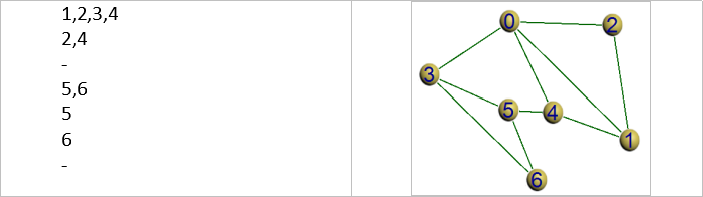
\includegraphics[width=1\textwidth]{AM/4}
	\caption{Пример представления неориентированного графа}
\end{figure}

\textcolor{black}{Признаком ориентированного графа является замена в последней строке файла знака “-“ на знак “+”; при
	этом строка, состоящая из единственного знака “-“, имеет смысл, аналогичный приведенному выше; элементами каждой
}\foreignlanguage{english}{\textit{\textcolor{black}{i}}}\textcolor{black}{{}-й строки, отличной от “-“ и “+“, могут
	быть как положительные, так и отрицательные числа
}\foreignlanguage{english}{\textit{\textcolor{black}{j}}}\textcolor{black}{, } $\left|j\right|>i$\textcolor{black}{:
}\foreignlanguage{english}{\textit{\textcolor{black}{j}}}\textcolor{black}{{\textgreater}0 - признак дуги
	(}\foreignlanguage{english}{\textit{\textcolor{black}{i}}}\textit{\textcolor{black}{,}}\foreignlanguage{english}{\textit{\textcolor{black}{j}}}\textcolor{black}{),
}\foreignlanguage{english}{\textit{\textcolor{black}{j}}}\textcolor{black}{{\textless}0 - признак дуги
	(}\foreignlanguage{english}{\textit{\textcolor{black}{j}}}\textit{\textcolor{black}{,}}\foreignlanguage{english}{\textit{\textcolor{black}{i}}}\textcolor{black}{).
	Текстовому файлу, приведенному на рис.~5.2 (слева), соответствует ориентированный граф из семи вершин (см. на рис.~5.2
	справа).}

\begin{figure}[H]
	\centering
	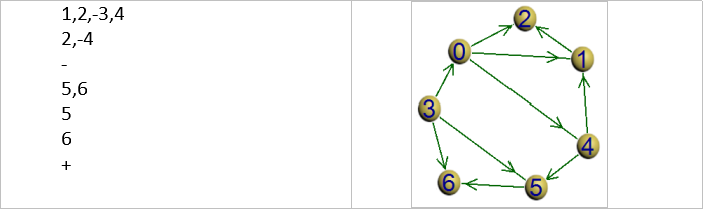
\includegraphics[width=1\textwidth]{AM/5}
	\caption{Пример представления ориентированного графа}
\end{figure}

\textcolor{black}{Не вдаваясь в подробное изложение вопросов распределения памяти, отметим, что объем требуемой памяти
	при описанном способе задания графа <<приближенно>> равен } $|E|$\textcolor{black}{, тогда как, например, все
	описанные в \cite[C. 203]{AKM_ch5_bib1} способы потребуют (для неориентированных графов) <<приближенно>> } $2|E|$
\textcolor{black}{\ памяти.}

\textcolor{black}{Набор исходных файлов, используемых в нашем
}\foreignlanguage{english}{\textcolor{black}{C}}\textcolor{black}{\#-проекте: 1) текстовый файл \linebreak
	“}\foreignlanguage{english}{\textcolor{black}{name}}\textcolor{black}{.}\foreignlanguage{english}{\textcolor{black}{txt}}\textcolor{black}{”
	со структурой описанного выше типа; 2) файл
	“}\foreignlanguage{english}{\textcolor{black}{name}}\textcolor{black}{.}\foreignlanguage{english}{\textcolor{black}{bmp}}\textcolor{black}{”
	с растровым рисунком для изображения вершин; 3) необязательный файл
	“}\foreignlanguage{english}{\textcolor{black}{coo}}\textcolor{black}{.}\foreignlanguage{english}{\textcolor{black}{txt}}\textcolor{black}{”,
	содержащий координаты вершин в последовательных строках. Если файл
	“}\foreignlanguage{english}{\textcolor{black}{coo}}\textcolor{black}{.}\foreignlanguage{english}{\textcolor{black}{txt}}\textcolor{black}{”
	существует, то координаты вершин загружаются из него, в противном случае координаты вершин графа генерируются
	автоматически, после чего вызывается функция (обозначим ее
}\foreignlanguage{english}{\textcolor{black}{Dr}}\textcolor{black}{) рисования графа.}

\textcolor{black}{Распространенной ошибкой при наборе чисел с разделительным знаком <<запятая>> является вставка
	избыточного знака пробела после запятой. Покажем, как средствами языка
}\foreignlanguage{english}{\textcolor{black}{C}}\textcolor{black}{\# достигается устойчивость к ошибкам такого рода
	(предполагается, что строковый массив }\foreignlanguage{english}{\textit{\textcolor{black}{t}}}\textcolor{black}{,
	массив }\foreignlanguage{english}{\textit{\textcolor{black}{p}}}\textcolor{black}{ с элементами класса Point и двумерный <<зубчатый>> целочисленный
	массив }\foreignlanguage{english}{\textit{\textcolor{black}{a}}}\textcolor{black}{, соответствующий описанной выше
	структуре входного текстового файла, уже объявлены ранее):}

\begin{verbatim}
	t = File.ReadAllLines(“name.txt”);
	n = t.Length; p = new Point[n]; a = new	int[n][];
	for (int i = 0; i < n; i++)
	{
		if ((t[i] == "-") || (t[i] == "+")) continue;
		a[i] = t[i].Split(',').Select(q => q.Trim()).Select(int.Parse).ToArray();
	}
\end{verbatim}
%\foreignlanguage{english}{\textcolor{black}{t = File.ReadAllLines(“name.txt”); }}
%
%\foreignlanguage{english}{\textcolor{black}{n = t.Length; p = new Point[n];
%}}\foreignlanguage{english}{\textit{\textcolor{black}{a}}}\foreignlanguage{english}{\textcolor{black}{ = new
%		int[n][];}}
%
%\foreignlanguage{english}{\textcolor{black}{for (int i = 0; i {\textless} n; i++)}}
%
%\foreignlanguage{english}{\textcolor{black}{\{}}
%
%\foreignlanguage{english}{\textcolor{black}{\ \ \ \ \ if ((t[i] == -) {\textbar}{\textbar}
%		(t[i] == +)) continue;}}
%
%\foreignlanguage{english}{\textcolor{black}{\ \ \ \ \ }}\foreignlanguage{english}{\textit{\textcolor{black}{a}}}\foreignlanguage{english}{\textcolor{black}{[i]
%		= t[i].Split(',').Select(q ={\textgreater} q.Trim()).Select(int.Parse).ToArray();}}
%
%\textcolor{black}{\}}

\textcolor{black}{Отметим здесь же, что на стадии инициализации рисунок из файла “name.bmp” вводится в объект b класса
	Bitmap, затем масштабируется (величина d, указанная ниже, может быть изменена интерактивным способом), его краям
	придается свойство прозрачности:}

\begin{verbatim}
Bitmap b = new Bitmap(name.bmp);
b = new Bitmap(b, d, d);
b.MakeTransparent().}
\end{verbatim}


%\foreignlanguage{english}{\textcolor{black}{Bitmap b = new Bitmap(name.bmp);}}
%
%\foreignlanguage{english}{\textcolor{black}{b = new Bitmap(b, d, d);}}
%
%\textcolor{black}{b.MakeTransparent().}

\section{Редактирование рисунка графа}\label{AKM_ch5_3}

\hypertarget{Toc503377151}{}\textcolor{black}{Как правило, следствием автоматической генерации координат вершин графа
}\textit{\textcolor{black}{p}}\textcolor{black}{[}\textit{\textcolor{black}{i}}\textcolor{black}{] - объектов класса
}\textit{\textcolor{black}{Point}}\textcolor{black}{ (}\textit{\textcolor{black}{i}}\textcolor{black}{=0, …,
}\textit{\textcolor{black}{n}}\textcolor{black}{{}-1) является рисунок, не вполне соответ}\textcolor{black}{ствующий
	целям автора. Поэтому в проекте необходимо предусмотреть визуальное перемещение вершин графа с помощью мышки: }

\noindent 1. В обработчике события

\begin{verbatim}
	pictureBox1_MouseDown(object sender, MouseEventArgs e)
\end{verbatim}

%{\centering
%	\foreignlanguage{english}{\textcolor{black}{pictureBox1\_MouseDown(object sender, MouseEventArgs e)}}
%	\par}

\noindent вычисляется индекс I вершины, ближайшей к точке (e.X, e.Y) нажатия кнопки мыши и устанавливается
	флажок нажатия - некоторой глобальной логической переменной присваивается значение
True (опускание флажка выполняется в обработчике
события pictureBox1\_MouseUp);

\noindent 2. В обработчике события перемещения мыши:

\begin{verbatim}
pictureBox1_MouseMove(object sender, MouseEventArgs e)
\end{verbatim}
%{\centering
%	\foreignlanguage{english}{\textcolor{black}{pictureBox1\_MouseMove(object sender, MouseEventArgs e)}}
%	\par}

\noindent проверяется факт установки флажка нажатия и, если флажок установлен, точка
\textit{\textcolor{black}{p}}\textcolor{black}{[I] воссоздается с текущими координатами курсора мыши:
}\textit{\textcolor{black}{p}}\textcolor{black}{[I] = new }\textit{\textcolor{black}{Point}}\textcolor{black}{(e.X,
	e.Y), после чего вызывается функция Dr для прорисовки графа.}

\textcolor{black}{Отметим две коллизии, возникающие при этом. Если фрагменты рисунка выводятся непосредственно на
	<<холст>> видимого окна (в нашем случае - окна графического контейнера
}
\foreignlanguage{english}{\textcolor{black}{pictureBox 1}}, то в промежутках между выводом этих
	фрагментов экран успевает обновиться, вследствие чего рисунок претерпевает искажения. Искажения такого рода в
	компьютерной терминологии называются \textit{\textcolor{black}{артефактами}}\textcolor{black}{. Для исключения
	появления артефактов рекомендуется использовать метод }\textit{\textcolor{black}{двойной
		буферизации}} \cite[C. 264]{AKM_ch5_bib2}. Для этих целей на стадии инициализации нашего проекта создается объект
\foreignlanguage{english}{\textcolor{black}{b}}\textcolor{black}{0 класса}\foreignlanguage{english}{\textcolor{black}{Bitmap}}\textcolor{black}{, размеры которого совпадают с размерами
	графического контейнера }\foreignlanguage{english}{\textcolor{black}{pictureBox}}\textcolor{black}{1:}

\begin{verbatim}
Bitmap b0 = new Bitmap (pictureBox1.Width, pictureBox1.Height);
\end{verbatim}

%\foreignlanguage{english}{\textcolor{black}{Bitmap b0= new Bitmap (pictureBox1.Width, pictureBox1.Height);}}

\noindent затем создаются два <<холста>> - объекты класса Graphics - g0 и g1, соответствующие объектам b0 и
	pictureBox1:

\begin{verbatim}
g0 = Graphics.FromImage(b0);
g1 = pictureBox1.CreateGraphics().
\end{verbatim}

%\foreignlanguage{english}{\textcolor{black}{g0 = Graphics.FromImage(b0);}}
%
%\foreignlanguage{english}{\textcolor{black}{g1 = pictureBox1.CreateGraphics().}}

\textcolor{black}{В упомянутой выше функции Dr процесс вывода всех частей рисунка выполняется прежде всего на холст g0
	объекта b0, выполняющего роль второго буфера: сначала вывод линий - со стрелками или без них, затем вывод изображения b в точках расположения вершин
	и, наконец, вывод номеров вершин (такая последовательность существенна).}

\textcolor{black}{В конце функции Dr, после завершения формирования рисунка графа на холсте g0 объекта b0, выполняется
	вывод b0 на холст g1 графического контейнера pictureBox1. Как известно, здесь возможны два варианта:}

\noindent\textcolor{black}{1) вызов метода DrawImage: }

\begin{verbatim}
g1.DrawImage(b0, 0,0)
\end{verbatim}
холста g1 графического контейнера pictureBox1

%\textcolor{black}{g1.DrawImage(b0, 0,0)\newline
%	холста g1 графического контейнера pictureBox1 }

\textcolor{black}{или\newline
	2) присвоение b0 свойству Image этого контейнера:}

\begin{verbatim}
pictureBox1.Image = b0.
\end{verbatim}
%\textcolor{black}{pictureBox1.Image = b0.}

\textcolor{black}{Мы рекомендуем второй вариант. Практика показывает неустойчивость вывода при первом варианте. Причины
	этой коллизии автору неизвестны.}

\begin{remark}
Специальные классы C\#, предназначенные для реализации метода двойной буферизации, подробно
	рассмотрены в статье \cite{AKM_ch5_bib3}.
\end{remark}

\noindent На рис.~\ref{akm5.3_pic}: слева - граф с вершинами, координаты которых сгенерированы программой (при отсутствии файла \foreignlanguage{english}{\textcolor{black}{"coo.txt"}}\textcolor{black}{),
	справа --- граф, преобразованный пользователем в интерактивном режиме; сохранение преобразованных координат вершин с
	целью выбора их из файла при очередном запуске программы не представляет труда.}

\begin{figure}[H]\label{akm5.3_pic}
	\centering
	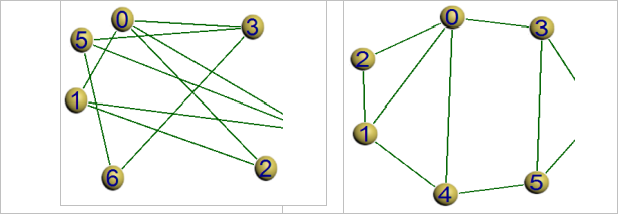
\includegraphics[width=1\textwidth]{AM/6}
	\caption{Пример визуальной перестройки графа.}
\end{figure}

\begin{remark}
Масштабирование рисунка в целом или отдельных его элементов --- радиуса фигуры, изображающей
	вершину, толщину линий (ребер, дуг), надписей (с сохранением координат вершин) --- достигается привязкой параметров этих
	элементов к свойству  Value визуальной
	компоненты \foreignlanguage{english}{\textit{\textcolor{black}{trackBar}}}.
\end{remark}
\noindent На рис.~\ref{akm5.4_pic} показан 	результат использования такой привязки.

\begin{figure}[H]\label{akm5.4_pic}
	\centering
	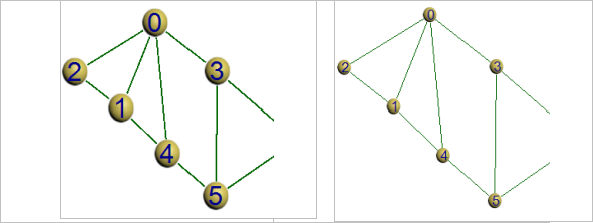
\includegraphics[width=1\textwidth]{AM/7}
	\caption{Визуальные элементы графа, изображенного слева, масштабированы за исключением координат вершин (результат см. справа).}
\end{figure}
Рассмотренная компактная структура исходного файла с информацией о графе
	допускает тривиальное обобщение на случай смешанного графа. Все приведенные в данном разделе рисунки созданы с помощью
C\#-проекта, описанию которого посвящено сообщение.

%\section{Заключение}\label{AKM_ch5_4}
%Рассмотренная компактная структура исходного файла с информацией о графе
%	допускает тривиальное обобщение на случай смешанного графа. Все приведенные в данном разделе рисунки созданы с помощью
%C\#-проекта, описанию которого посвящено сообщение.
%
%\textcolor{black}{Результаты раздела опубликованы в \cite{AKM_ch5_bib4} --\cite{AKM_ch5_bib5}.}








%%%%%%%%%%%%%%%%%%%%%%%%%%%
%%%%%%%%%%%%%%%%%%%%%%%%%%%
%%%%%%%%%%%%%%%%%%%%%%%%%%%

